\documentclass[a4paper]{article}

% CJK support: prefer ctex, fallback to XeTeX native line breaking
\IfFileExists{ctex.sty}{
  \usepackage[fontset=fandol]{ctex}
}{
  % Fallback for minimal TeX installs (e.g. MacTeX Basic, TeX Live scheme-basic)
  % without ctex/xeCJK. Uses XeTeX's built-in CJK line breaking.
  \usepackage{fontspec}
  \XeTeXlinebreaklocale "zh"
  \XeTeXlinebreakskip = 0pt plus 1pt
  \IfFontExistsTF{Songti SC}{\setmainfont{Songti SC}}{%
    \IfFontExistsTF{Noto Serif CJK SC}{\setmainfont{Noto Serif CJK SC}}{}%
  }
  \IfFontExistsTF{Heiti SC}{\setsansfont{Heiti SC}}{%
    \IfFontExistsTF{Noto Sans CJK SC}{\setsansfont{Noto Sans CJK SC}}{}%
  }
}

% Basic packages
\usepackage{amsmath, amssymb}
\usepackage{graphicx}
\usepackage[margin=2.5cm]{geometry}
\emergencystretch=3em
\usepackage[most]{tcolorbox}
\usepackage{etoolbox}
\usepackage{listings}
\usepackage{hyperref}
\usepackage{booktabs}
\usepackage{array}
\usepackage{subcaption}
\usepackage{float}
\usepackage{tikz}
\IfFileExists{pgfplots.sty}{
    \usepackage{pgfplots}
    \pgfplotsset{compat=1.18}
}{}

% ===== Highlight boxes =====
\newtcolorbox{knowledgebox}[1]{
    enhanced, colback=blue!5!white, colframe=blue!75!black, colbacktitle=blue!75!black,
    coltitle=white, fonttitle=\bfseries, title={#1}, attach boxed title to top left={yshift=-2mm, xshift=2mm},
    boxrule=1pt, sharp corners
}

\newtcolorbox{importantbox}[1]{
    enhanced, colback=yellow!10!white, colframe=yellow!80!black, colbacktitle=yellow!80!black,
    coltitle=black, fonttitle=\bfseries, title={#1}, sharp corners
}

\newtcolorbox{warningbox}[1]{
    enhanced, colback=red!5!white, colframe=red!75!black, colbacktitle=red!75!black,
    coltitle=white, fonttitle=\bfseries, title={#1}, sharp corners
}

\newtcolorbox{practicebox}[1]{
    enhanced, colback=black!3!white, colframe=black!75, colbacktitle=black!75,
    coltitle=white, fonttitle=\bfseries, title={#1}, sharp corners
}

% ===== Code listings =====
\lstset{
    basicstyle=\ttfamily\small,
    keywordstyle=\color{blue},
    stringstyle=\color{red!60!black},
    commentstyle=\color{green!60!black},
    breaklines=true,
    frame=single,
    numbers=left,
    numberstyle=\tiny\color{gray},
    captionpos=b,
    extendedchars=false
}

% ===== Figure provenance and unit macros =====
% \vtag goes inside \caption{...}; \srcnote{MM:SS--MM:SS} follows the figure environment.
\newcommand{\vtag}{\protect\footnotemark}
\newcommand{\srcnote}[1]{\footnotetext{视频画面时间区间：#1。若为裁剪图，时间区间仍对应原视频画面。}}
% Units work in text and math mode; never hand-write $^\circ$ or \AA inside \mathrm.
\newcommand{\degC}{\ensuremath{^{\circ}\mathrm{C}}}
\newcommand{\um}{\ensuremath{\mu\mathrm{m}}}
\newcommand{\nm}{\ensuremath{\mathrm{nm}}}
\newcommand{\angstrom}{\ensuremath{\text{\AA}}}

% ===== Front-page metadata =====
% Fill these in when generating notes.
\newcommand{\notetitle}{优化基础}
\newcommand{\notesubtitle}{GAMES001 图形学中的数学 · 第 15 集：无约束优化、拉格朗日乘子与对偶}
\newcommand{\noteauthors}{根据 GAMES-Webinar 直播录像整理（阮良旺 主讲）}
\newcommand{\notedate}{2024年6月24日（直播）}
\newcommand{\videochannel}{GAMES-Webinar（哔哩哔哩）}
\newcommand{\videopublishdate}{2024年3月6日（合集）}
\newcommand{\videoduration}{1小时33分22秒}
\newcommand{\videourl}{https://www.bilibili.com/video/BV1MF4m1V7e3/?p=15}
\newcommand{\videocoverpath}{cover.jpg}

\begin{document}

% ===== Title page =====
\begin{titlepage}
\centering
{\Large 课程笔记\par}
\vspace{1.2cm}
{\huge\bfseries \notetitle\par}
\ifdefempty{\notesubtitle}{}{
\vspace{0.3cm}
{\large \notesubtitle\par}
}
\vspace{0.5cm}
{\large \noteauthors\par}
\vspace{0.3cm}
{\large \notedate\par}
\vspace{1.0cm}

\ifdefempty{\videocoverpath}{
{\small 请在生成笔记时填入视频封面图的本地路径。\par}
}{
\includegraphics[width=0.82\textwidth,height=0.40\textheight,keepaspectratio]{\videocoverpath}\par
}

\vfill
\begin{tcolorbox}[width=0.9\textwidth, colback=black!2!white, colframe=black!60, sharp corners]
\textbf{视频作者/频道}：\videochannel\par
\textbf{发布日期}：\videopublishdate\par
\textbf{视频时长}：\videoduration\par
\textbf{视频链接}：
\ifdefempty{\videourl}{
未填写
}{
\href{\videourl}{\nolinkurl{\videourl}}
}
\end{tcolorbox}
\end{titlepage}

\tableofcontents
\newpage

%% --- 正文内容开始 --- %%

\section{这一讲讲什么}

第十五集对应课程的第十四讲，题目是“优化基础”，由北京大学的阮良旺主讲。讲者开场就说，优化本身是一个涵盖内容非常多、同时也非常难的大学科，课件上摆了好几本厚厚的优化教材；而今天只有一个多小时，肯定没法讲得特别详细。所以他的目标是尽可能用一节课的时间，给大家看一看优化里面大家经常用到的概念和算法。

\noindent\begin{minipage}{\textwidth}
\begin{figure}[H]
\centering

\includegraphics[width=0.92\textwidth]{figures/fig_01_big_topic.jpg}
\caption{优化是一个宏大的课题\vtag}
\end{figure}
\srcnote{00:06:00--00:06:15}
\end{minipage}


本讲分为两大部分。第一部分是无约束优化：从最小二乘、曲面参数化、弹性体模拟三个例子说明图形学里到处都是优化问题，然后介绍线搜索框架下的梯度下降、牛顿迭代和拟牛顿法，重点是 BFGS 与 L-BFGS，并回顾上一讲的不动点迭代也是一种拟牛顿法。第二部分是带约束优化：从等式约束的最优条件出发，引入拉格朗日乘子，把问题写成 min-max 博弈，介绍用牛顿法求解拉格朗日函数、对偶问题、对偶上升法和罚函数法，最后简单提一下不等式约束。

\section{优化问题}

\noindent\begin{minipage}{\textwidth}
\begin{figure}[H]
\centering
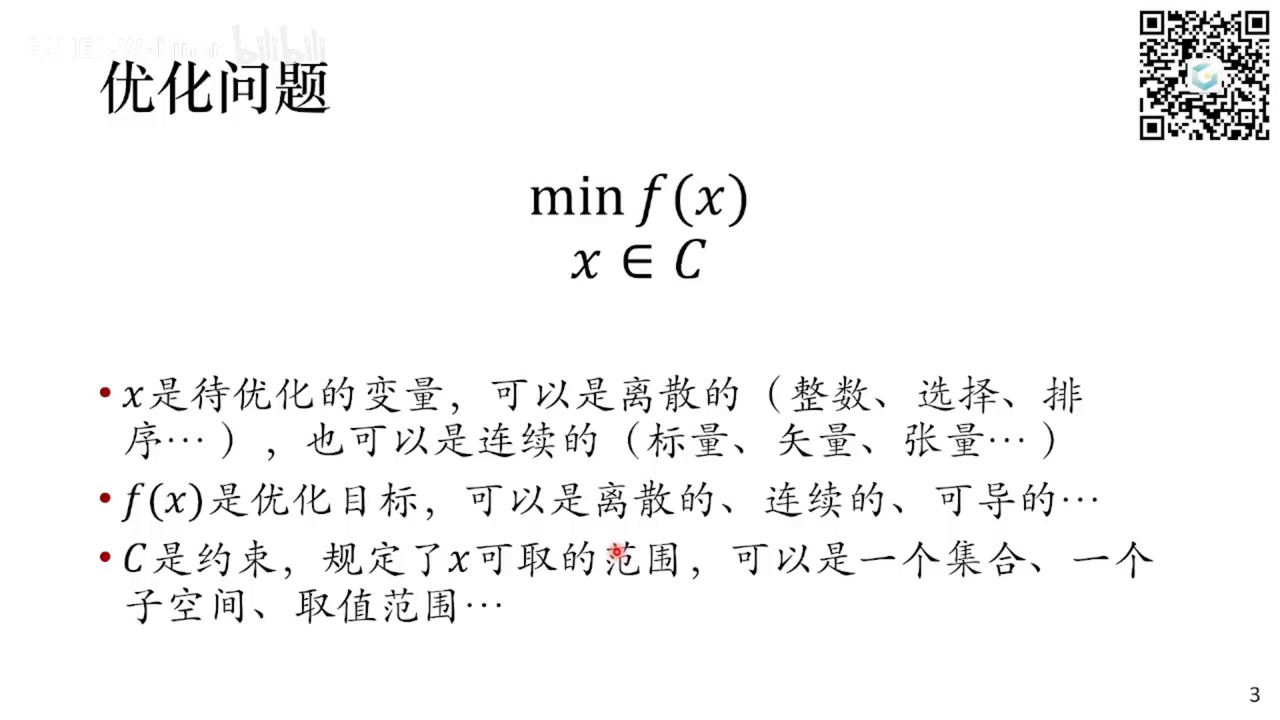
\includegraphics[width=0.92\textwidth]{figures/fig_02_problem.jpg}
\caption{优化问题的一般形式\vtag}
\end{figure}
\srcnote{00:07:00--00:07:15}
\end{minipage}


一个优化问题可以写成比较通用的形式
\begin{equation}
\min_{x\in C} f(x).
\end{equation}
其中：
\begin{itemize}
\item $x$ 是待优化的变量，可以是离散的（整数、选择、排序等），也可以是连续的（标量、矢量、张量等）；
\item $f(x)$ 是优化目标，可以是离散的、连续的、可导的等等；
\item $C$ 是约束，规定了 $x$ 可取的范围，可以是一个集合、一个子空间、一个取值范围。
\end{itemize}
讲者说，具体用什么方法求解，要根据问题的具体形式去决定。

\begin{importantbox}{本讲覆盖的两类问题}
今天只讨论 $x$ 是连续向量、$f$ 连续可微的情形，分两类：一是 $C=\mathbb R^n$ 的无约束优化，核心是怎样选下降方向和步长；二是带等式约束的优化，核心是拉格朗日函数和对偶。离散优化、凸优化理论、不等式约束的完整处理都不在本讲范围内。
\end{importantbox}

\section{无约束优化与三个例子}

\noindent\begin{minipage}{\textwidth}
\begin{figure}[H]
\centering
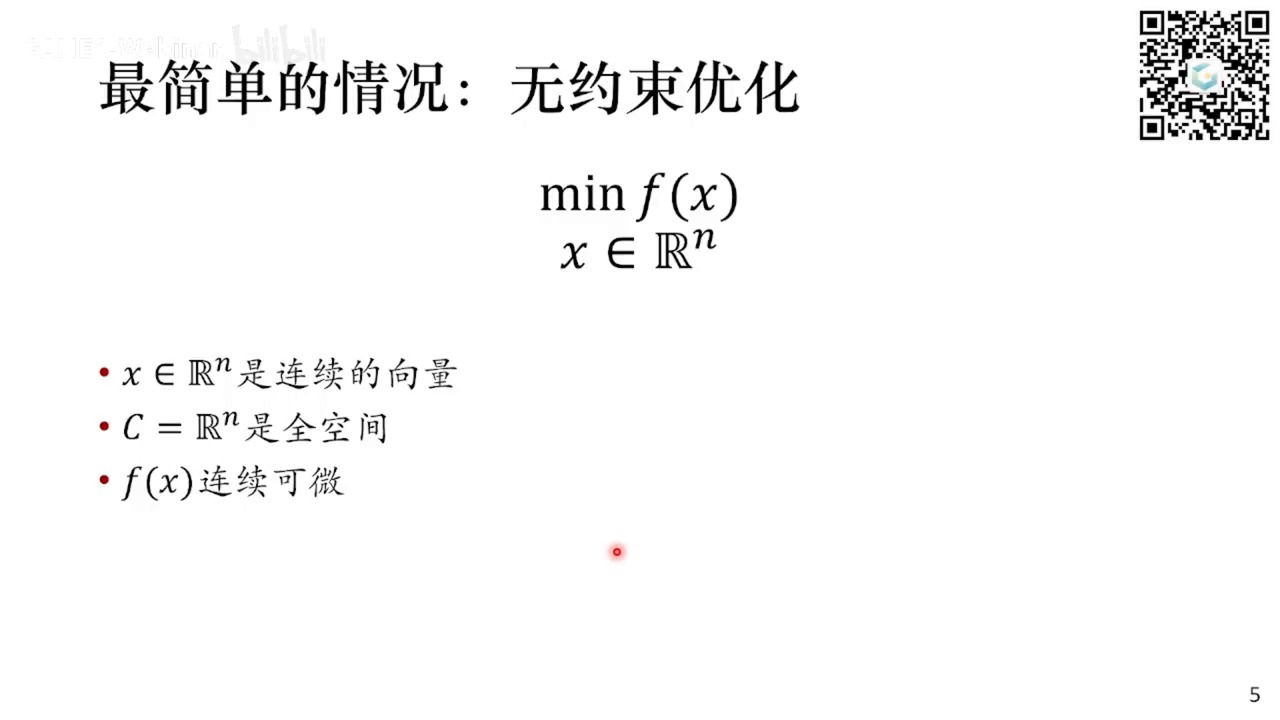
\includegraphics[width=0.92\textwidth]{figures/fig_03_unconstrained.jpg}
\caption{最简单的情况：无约束优化\vtag}
\end{figure}
\srcnote{00:07:30--00:07:45}
\end{minipage}


最简单的情况是无约束优化：
\begin{equation}
\min_{x\in\mathbb R^n} f(x),
\end{equation}
其中 $x\in\mathbb R^n$ 是连续的向量，$C=\mathbb R^n$ 是全空间，并且额外假设 $f(x)$ 连续可微。讲者先举了三个图形学里的例子，说明这样的问题无处不在。

\subsection{最小二乘法}

\noindent\begin{minipage}{\textwidth}
\begin{figure}[H]
\centering
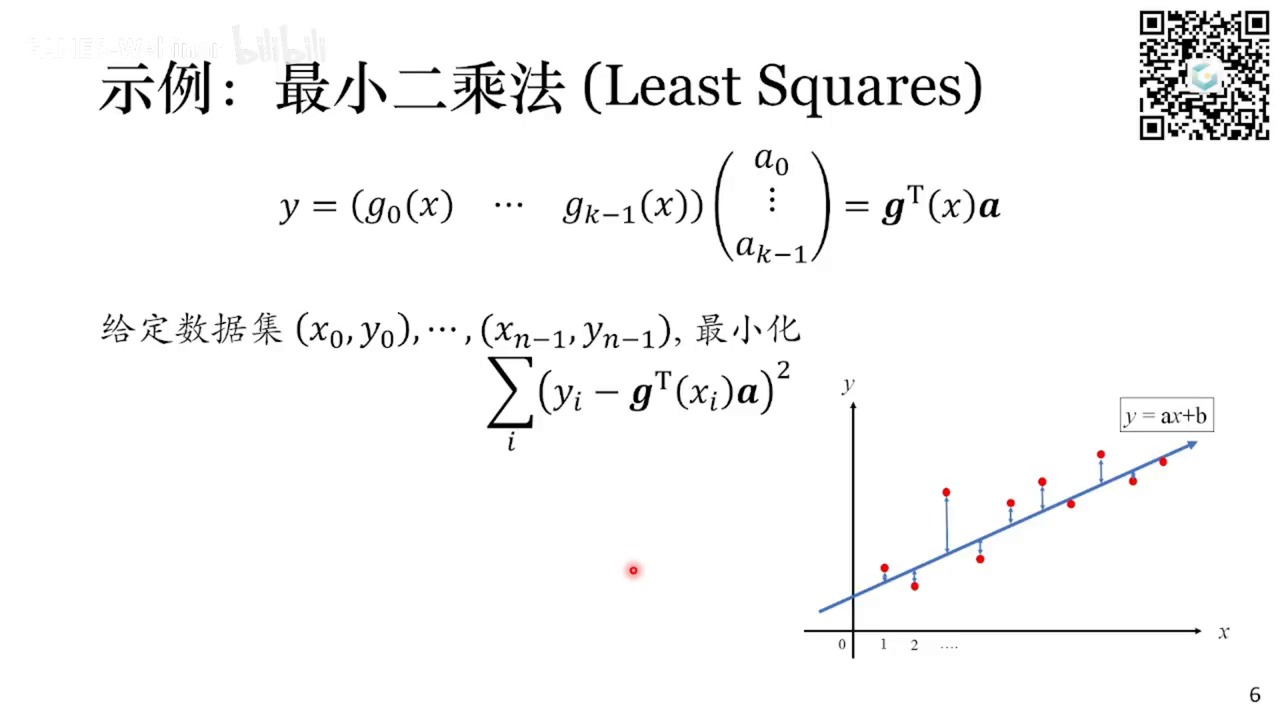
\includegraphics[width=0.92\textwidth]{figures/fig_04_lsq1.jpg}
\caption{示例：最小二乘法的模型\vtag}
\end{figure}
\srcnote{00:09:00--00:09:15}
\end{minipage}


第一个例子是大家最熟悉的最小二乘法。我们希望拟合出一条曲线，假设 $y$ 与 $x$ 之间满足
\begin{equation}
y=\begin{pmatrix}g_0(x)&\cdots&g_{k-1}(x)\end{pmatrix}\begin{pmatrix}a_0\\ \vdots\\ a_{k-1}\end{pmatrix}=\boldsymbol g^{\mathrm T}(x)\boldsymbol a,
\end{equation}
其中 $g_0,\dots,g_{k-1}$ 是给定的基函数，比如常数、一次函数、二次函数，$a_0,\dots,a_{k-1}$ 是待定系数。给定数据集 $(x_0,y_0),\dots,(x_{n-1},y_{n-1})$，最小化
\begin{equation}
\sum_i\left(y_i-\boldsymbol g^{\mathrm T}(x_i)\boldsymbol a\right)^2 .
\end{equation}

\noindent\begin{minipage}{\textwidth}
\begin{figure}[H]
\centering
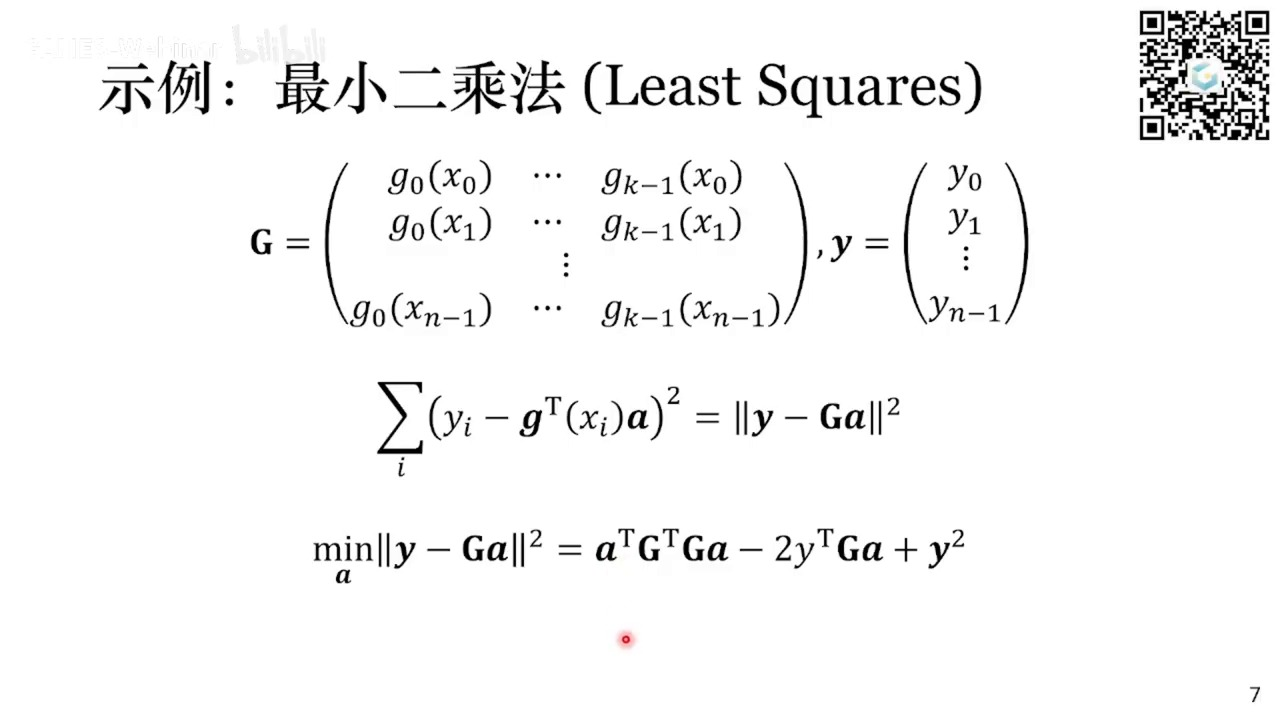
\includegraphics[width=0.92\textwidth]{figures/fig_05_lsq2.jpg}
\caption{示例：最小二乘法的矩阵形式\vtag}
\end{figure}
\srcnote{00:09:45--00:10:00}
\end{minipage}


把所有基函数在各个数据点上的值排成矩阵 $\mathbf G$，其中第 $i$ 行是 $\boldsymbol g^{\mathrm T}(x_i)$，所有 $y_i$ 排成向量 $\boldsymbol y$，优化目标可以写成更紧凑的形式
\begin{equation}
\min_{\boldsymbol a}\|\boldsymbol y-\mathbf G\boldsymbol a\|^2=\boldsymbol a^{\mathrm T}\mathbf G^{\mathrm T}\mathbf G\boldsymbol a-2\boldsymbol y^{\mathrm T}\mathbf G\boldsymbol a+\boldsymbol y^{\mathrm T}\boldsymbol y .
\end{equation}
这是关于 $\boldsymbol a$ 的二次函数。

\begin{knowledgebox}{最小二乘的解}
讲义作者补充：对上式求梯度并令其为零，得到正规方程 $\mathbf G^{\mathrm T}\mathbf G\boldsymbol a=\mathbf G^{\mathrm T}\boldsymbol y$。当 $\mathbf G$ 列满秩时 $\mathbf G^{\mathrm T}\mathbf G$ 正定，解唯一。这个例子也说明二次型目标的海森矩阵是常数矩阵 $2\mathbf G^{\mathrm T}\mathbf G$，后面讲牛顿法时会看到，对这种目标牛顿法一步就收敛。
\end{knowledgebox}

\subsection{曲面参数化}

\noindent\begin{minipage}{\textwidth}
\begin{figure}[H]
\centering
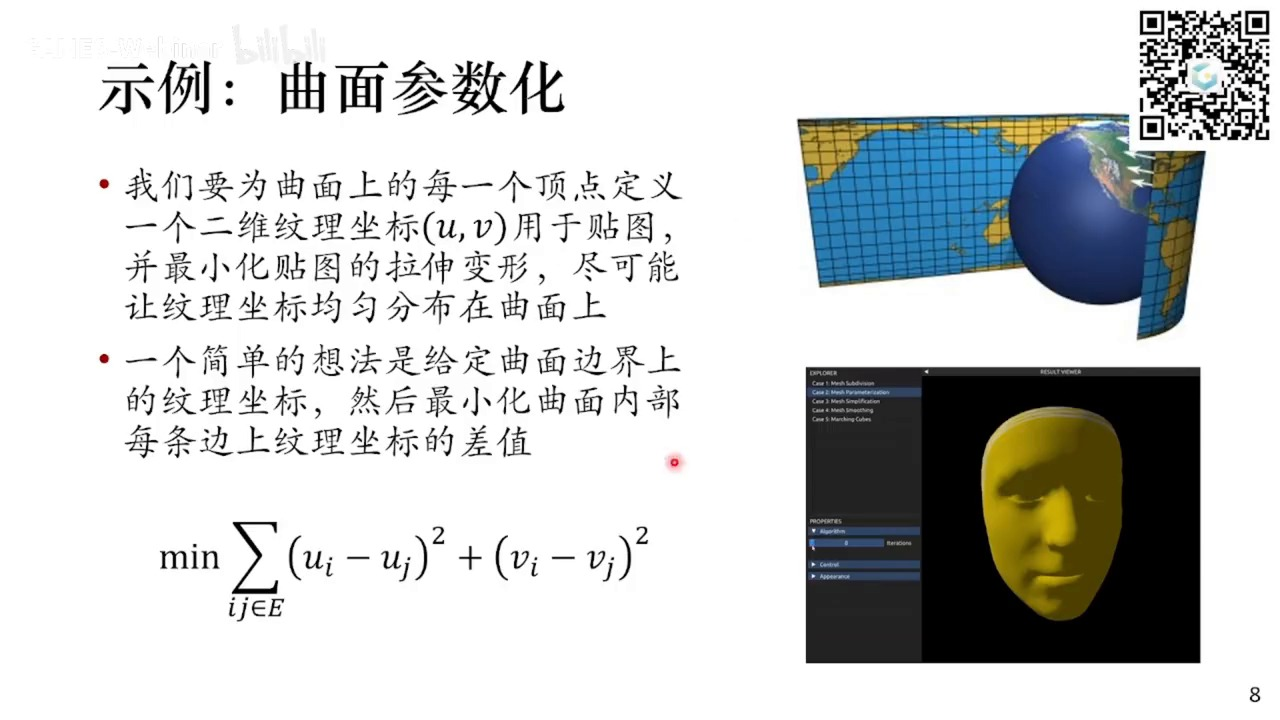
\includegraphics[width=0.92\textwidth]{figures/fig_06_param1.jpg}
\caption{示例：曲面参数化，为每个顶点定义纹理坐标\vtag}
\end{figure}
\srcnote{00:10:00--00:10:15}
\end{minipage}


第二个例子是曲面参数化。比如有一个用网格表示的球，要给它定义二维的纹理坐标 $(u,v)$，也叫 UV 坐标。讲者解释，可以把它理解成球面上的点与一张二维贴图之间的对应关系，有了它就能把贴图贴到曲面上。问题是：对任意的三维网格，比如课件上的人脸，要怎样确定每个顶点上的 UV 坐标，使得贴图贴到人脸上之后拉伸变形尽可能小、纹理坐标尽可能均匀地分布在曲面上？

\noindent\begin{minipage}{\textwidth}
\begin{figure}[H]
\centering
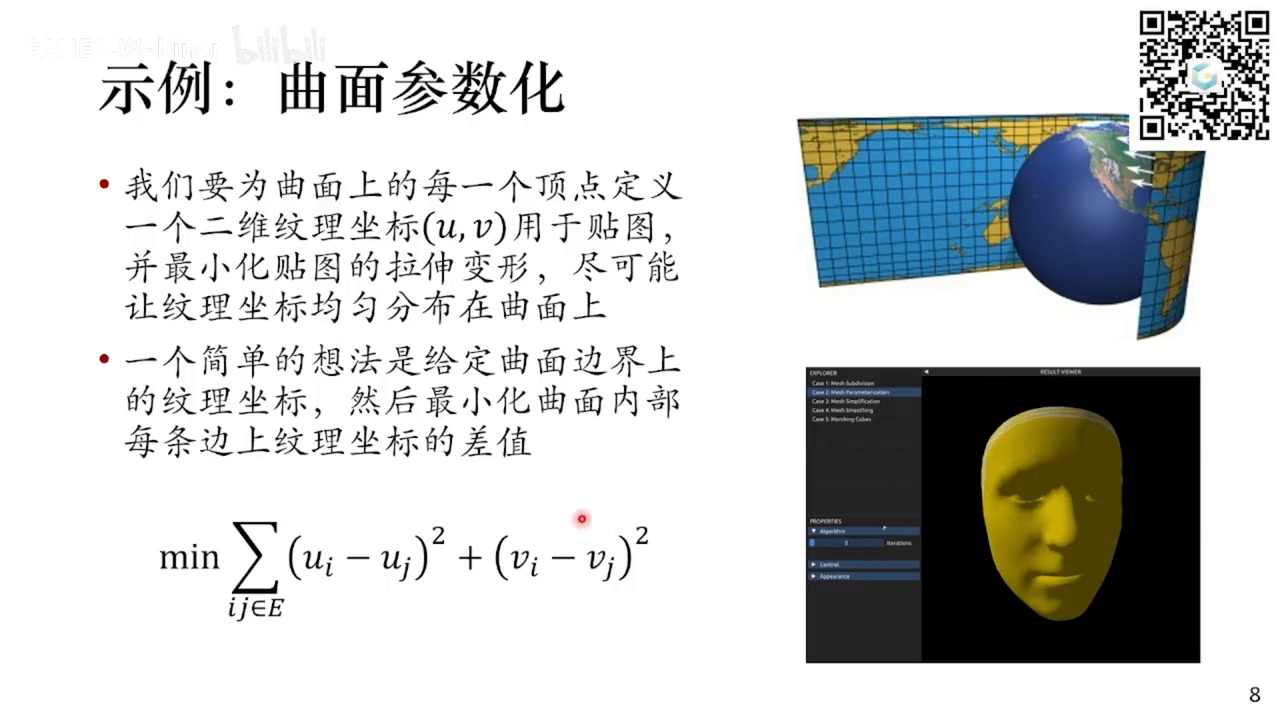
\includegraphics[width=0.92\textwidth]{figures/fig_07_param2.jpg}
\caption{给定边界纹理坐标，最小化内部每条边的差值\vtag}
\end{figure}
\srcnote{00:11:45--00:12:00}
\end{minipage}


一个简单的想法是：给定曲面边界上的纹理坐标，然后对网格上的每条边，要求两个顶点的 UV 坐标之差尽可能小：
\begin{equation}
\min\sum_{ij\in E}(u_i-u_j)^2+(v_i-v_j)^2 .
\end{equation}

\noindent\begin{minipage}{\textwidth}
\begin{figure}[H]
\centering
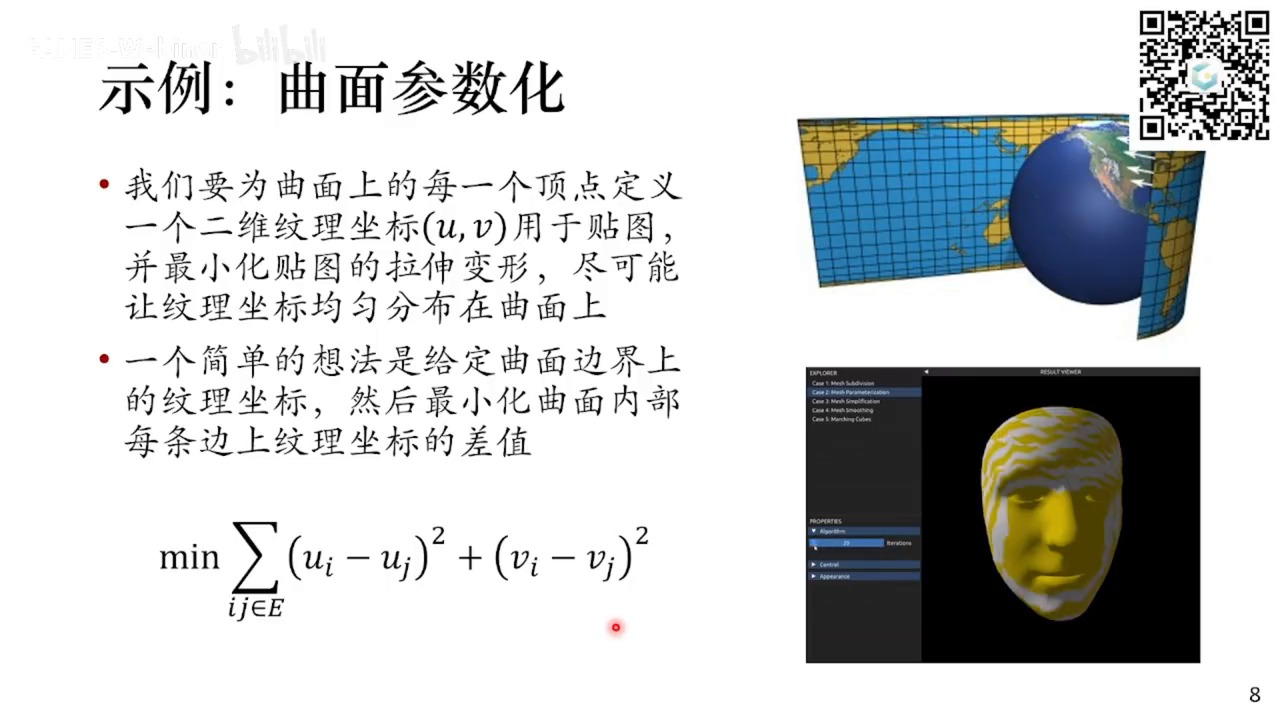
\includegraphics[width=0.92\textwidth]{figures/fig_08_param3.jpg}
\caption{参数化结果：纹理贴到人脸上的效果\vtag}
\end{figure}
\srcnote{00:12:45--00:13:00}
\end{minipage}


\begin{knowledgebox}{这个目标的最优条件}
讲义作者补充：对 $u_i$ 求导并令其为零，得到 $u_i=\frac{1}{|N(i)|}\sum_{j\in N(i)}u_j$，即每个内部顶点的坐标是邻居的平均。这正是第十三讲中拉普拉斯方程的离散形式，所以这类参数化（常称 Tutte 嵌入）最终归结为求解一个稀疏线性方程组。
\end{knowledgebox}

\subsection{弹性体模拟}

\noindent\begin{minipage}{\textwidth}
\begin{figure}[H]
\centering
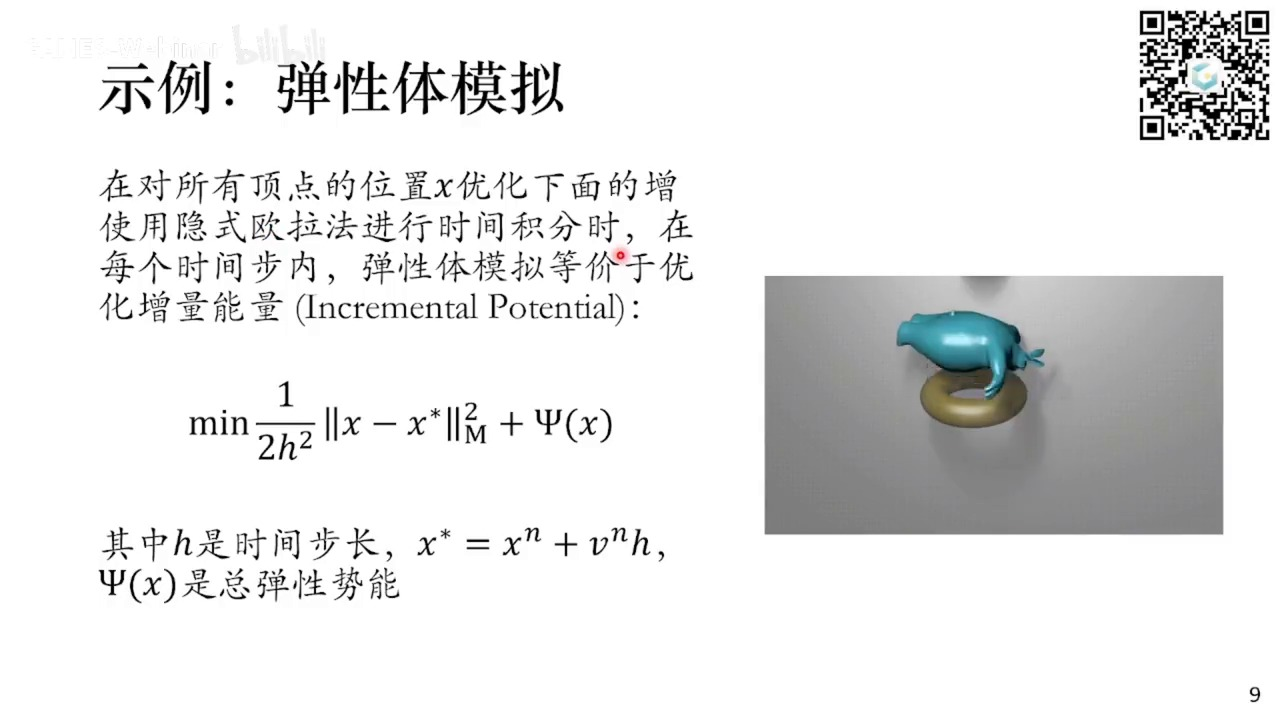
\includegraphics[width=0.92\textwidth]{figures/fig_09_elastic1.jpg}
\caption{示例：弹性体模拟的增量能量\vtag}
\end{figure}
\srcnote{00:13:00--00:13:15}
\end{minipage}


第三个例子是弹性体模拟。使用隐式欧拉法进行时间积分时，在每个时间步内，弹性体模拟等价于对所有顶点的位置 $x$ 优化下面的增量能量（incremental potential）：
\begin{equation}
\min_x\ \frac{1}{2h^2}\|x-x^*\|_M^2+\Psi(x),\qquad x^*=x^n+v^nh .
\end{equation}
其中 $h$ 是时间步长，$\Psi(x)$ 是总弹性势能。讲者解释，第一项叫惯性项，第二项是弹性势能。

\noindent\begin{minipage}{\textwidth}
\begin{figure}[H]
\centering
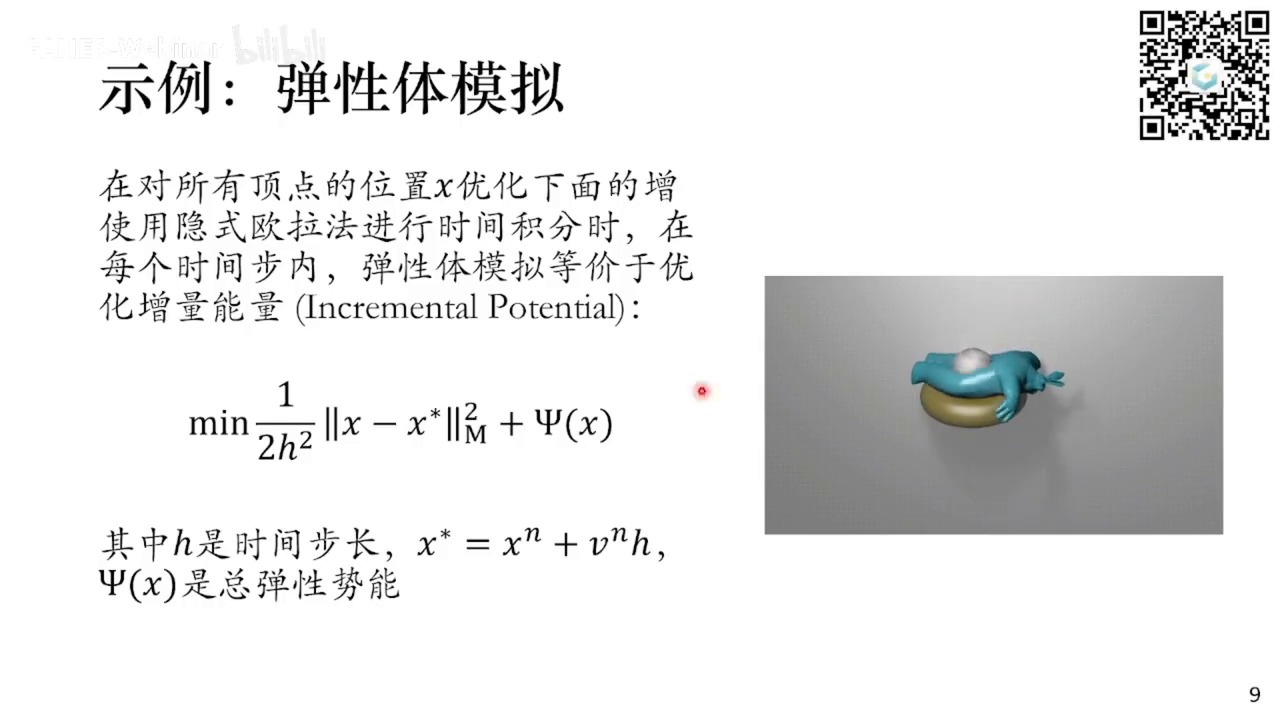
\includegraphics[width=0.92\textwidth]{figures/fig_10_elastic2.jpg}
\caption{弹性体模拟的效果\vtag}
\end{figure}
\srcnote{00:13:45--00:14:00}
\end{minipage}


\begin{knowledgebox}{为什么隐式欧拉等价于优化}
讲义作者补充：对增量能量求梯度并令其为零，得到 $M(x-x^n-v^nh)/h^2=-\nabla\Psi(x)$，也就是 $M\frac{v^{n+1}-v^n}{h}=-\nabla\Psi(x^{n+1})$，$v^{n+1}=(x^{n+1}-x^n)/h$，这正是隐式欧拉法的更新。把求解非线性方程改写成最小化能量的好处是，可以用线搜索保证每一步能量下降，求解更稳健。
\end{knowledgebox}

\section{线搜索与梯度下降}

\subsection{线搜索框架}

\noindent\begin{minipage}{\textwidth}
\begin{figure}[H]
\centering
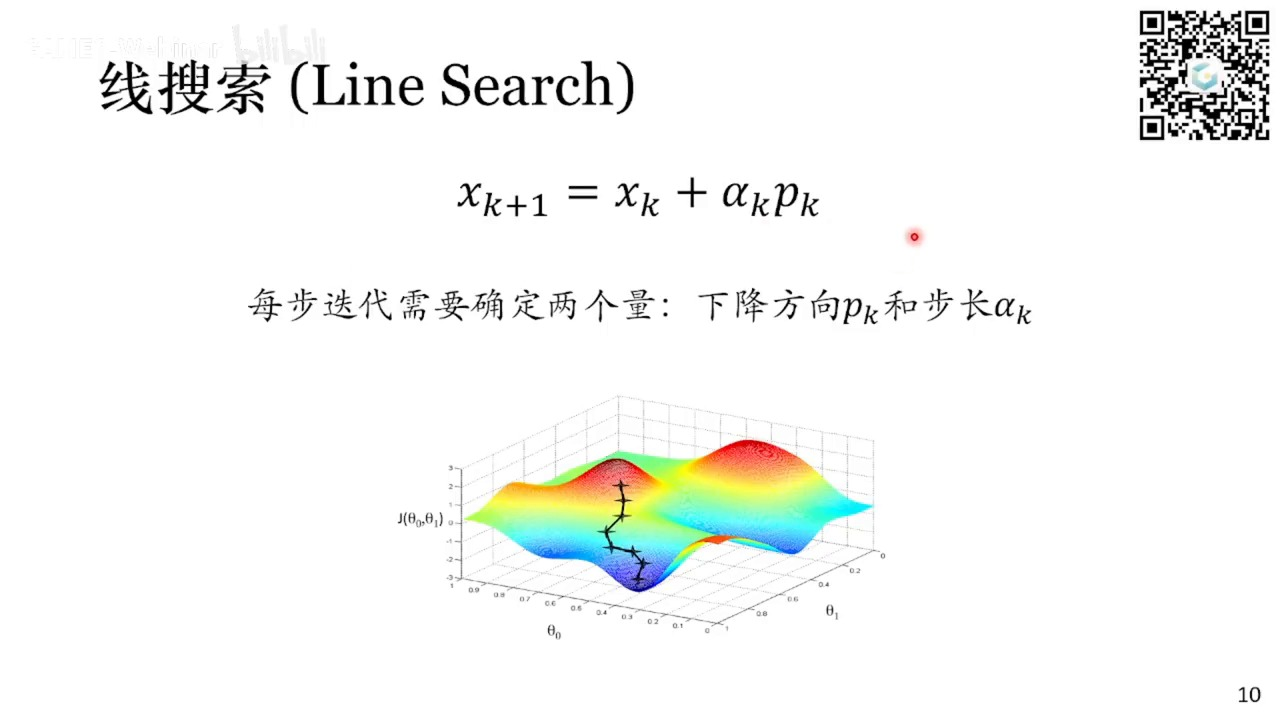
\includegraphics[width=0.92\textwidth]{figures/fig_11_line_search.jpg}
\caption{线搜索：每步迭代确定下降方向和步长\vtag}
\end{figure}
\srcnote{00:15:00--00:15:15}
\end{minipage}


对于这样的优化问题怎么求解？最简单的是线搜索（line search）类方法。设想一个很复杂的函数曲面，我们从某个点出发，每一步沿某个方向走一段距离：
\begin{equation}
x_{k+1}=x_k+\alpha_kp_k .
\end{equation}
每步迭代需要确定两个量：下降方向 $p_k$ 和步长 $\alpha_k$，也就是往哪个方向走、走多远。一直迭代下去，希望最终收敛到最优解。

\subsection{梯度下降}

\noindent\begin{minipage}{\textwidth}
\begin{figure}[H]
\centering
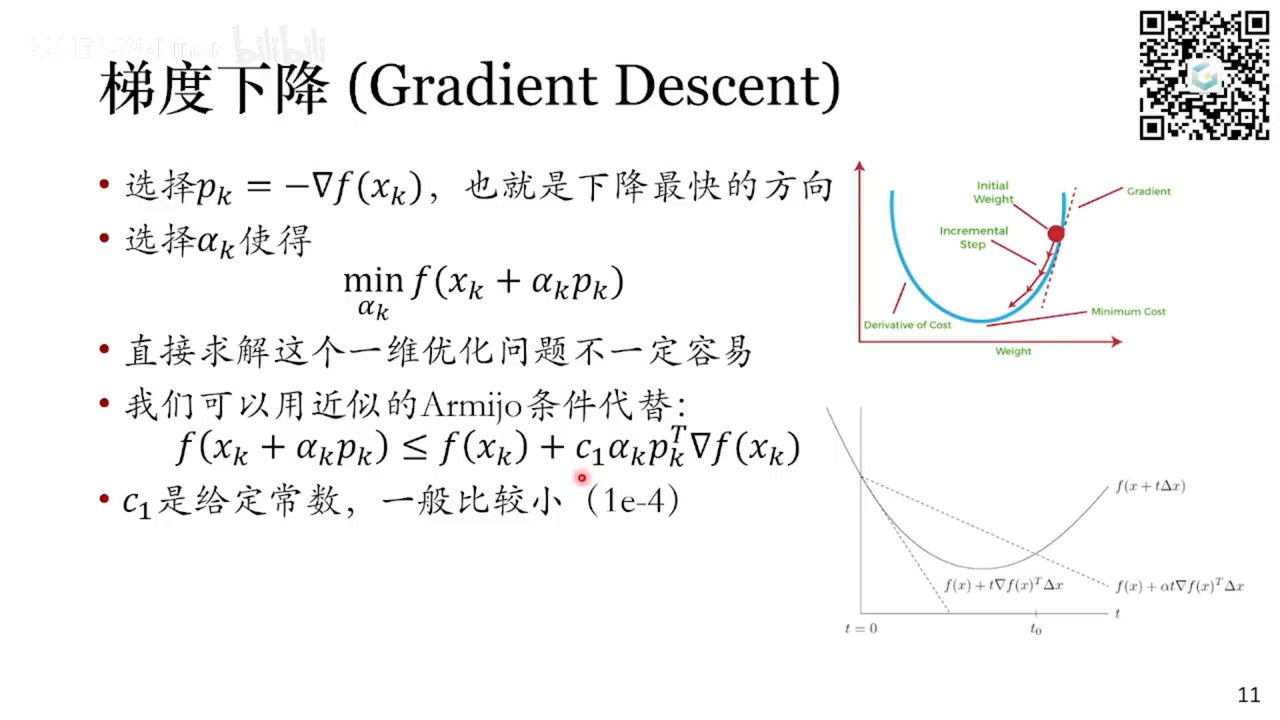
\includegraphics[width=0.92\textwidth]{figures/fig_12_gd.jpg}
\caption{梯度下降：沿负梯度方向\vtag}
\end{figure}
\srcnote{00:17:15--00:17:30}
\end{minipage}


梯度下降（gradient descent）选择 $p_k=-\nabla f(x_k)$，也就是下降最快的方向。步长 $\alpha_k$ 理想的选择是使得
\begin{equation}
\min_{\alpha_k}f(x_k+\alpha_kp_k).
\end{equation}
讲者说这是很自然的策略，但直接求解这个一维优化问题不一定容易：每一步迭代里还要套一个子迭代，整个算法会变慢。我们可以用近似的 Armijo 条件代替：
\begin{equation}
f(x_k+\alpha_kp_k)\le f(x_k)+c_1\alpha_kp_k^{\mathrm T}\nabla f(x_k),
\end{equation}
其中 $c_1$ 是给定的常数，一般比较小，比如 $10^{-4}$。

\subsection{Armijo 条件的含义}

\noindent\begin{minipage}{\textwidth}
\begin{figure}[H]
\centering
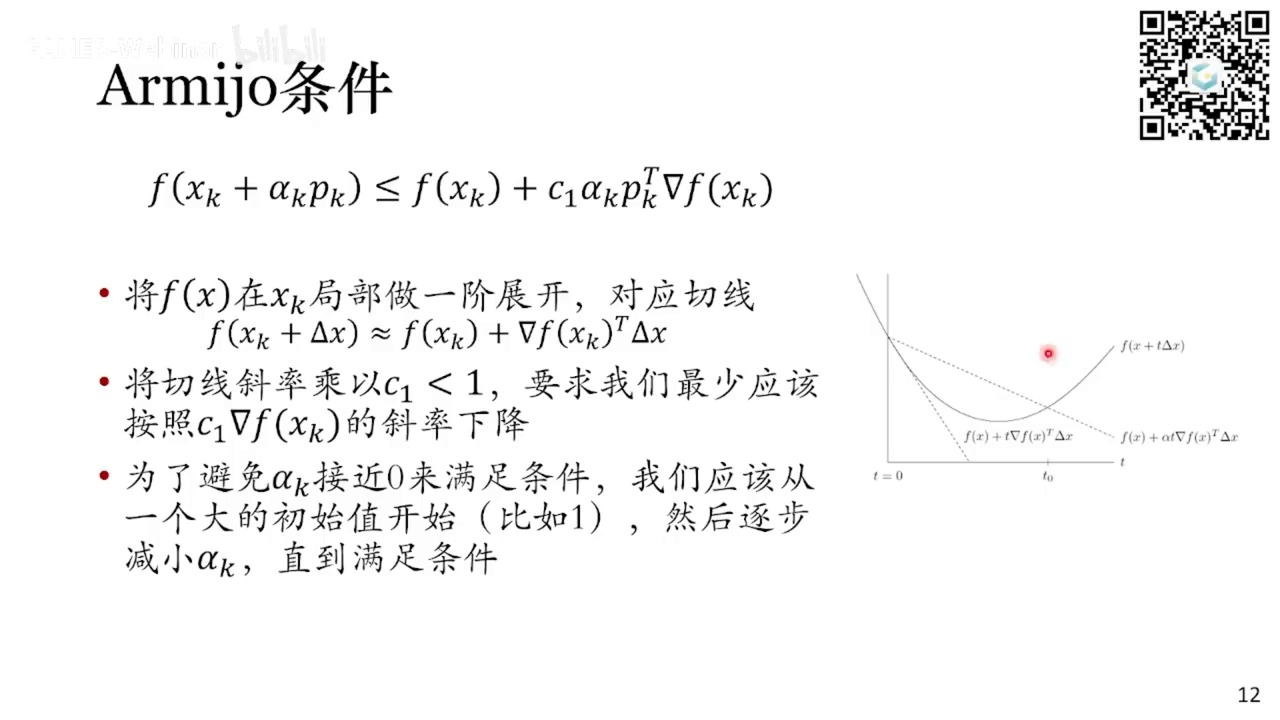
\includegraphics[width=0.92\textwidth]{figures/fig_13_armijo.jpg}
\caption{Armijo 条件的几何意义：放缓斜率的切线\vtag}
\end{figure}
\srcnote{00:21:00--00:21:15}
\end{minipage}


将 $f(x)$ 在 $x_k$ 处做一阶展开，对应切线
\begin{equation}
f(x_k+\Delta x)\approx f(x_k)+\nabla f(x_k)^{\mathrm T}\Delta x .
\end{equation}
把切线斜率乘以 $c_1<1$，Armijo 条件要求函数值至少要按照 $c_1\nabla f(x_k)$ 的斜率下降。讲者在图上解释：如果 $\alpha_k$ 取得太大，点就跑到放缓的切线上面去了，下降得不够多；合理的 $\alpha_k$ 只能在放缓切线下面的那一段。

为了避免 $\alpha_k$ 取到接近零来满足条件（那样几乎不动，条件总是成立），应该从一个大的初始值开始，比如 $1$，然后逐步减小 $\alpha_k$，直到满足条件。讲者举例：从 $\alpha=1$ 开始，发现跑太远了，就直接取一半，取一半发现正好跑到了放缓切线下面，就停下来，走对应的步长。这种做法常称为回溯线搜索。

\noindent\begin{minipage}{\textwidth}
\begin{figure}[H]
\centering
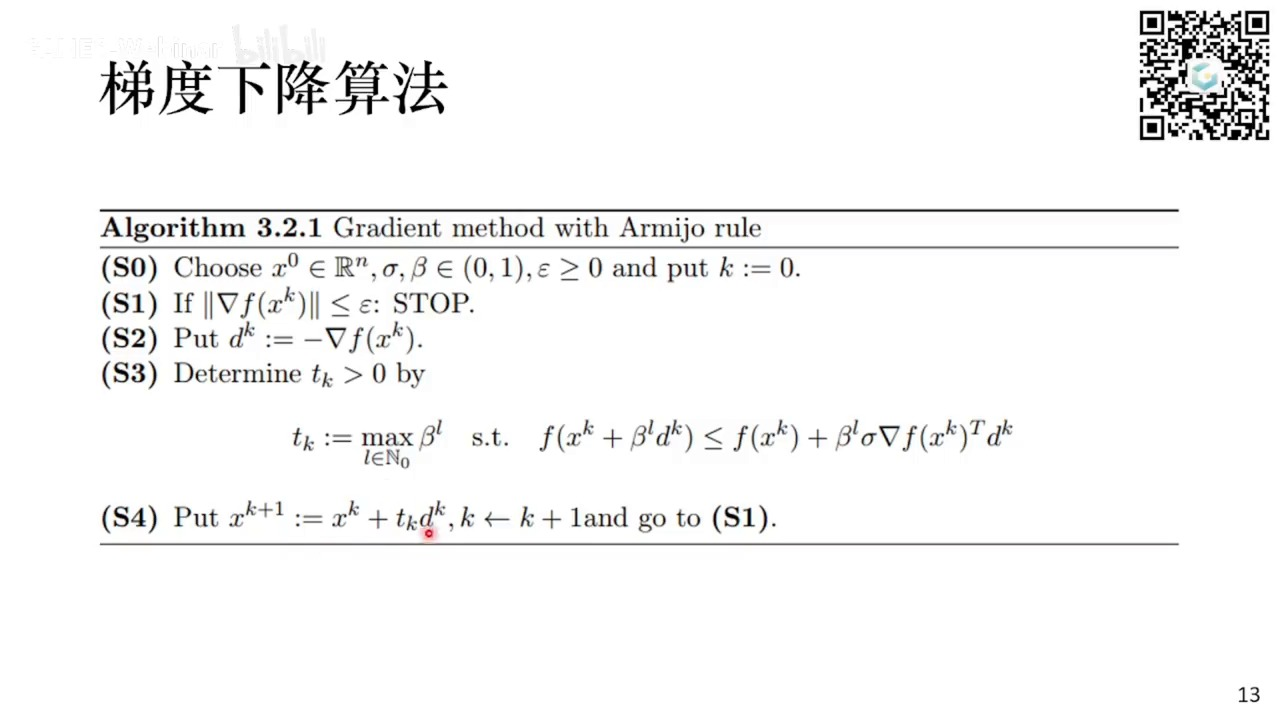
\includegraphics[width=0.92\textwidth]{figures/fig_14_gd_algo.jpg}
\caption{梯度下降算法\vtag}
\end{figure}
\srcnote{00:21:30--00:21:45}
\end{minipage}


\begin{practicebox}{回溯线搜索的伪代码}
讲义作者整理：给定 $x_k$，令 $p_k=-\nabla f(x_k)$，$\alpha=1$；当 $f(x_k+\alpha p_k)>f(x_k)+c_1\alpha p_k^{\mathrm T}\nabla f(x_k)$ 时令 $\alpha\leftarrow\alpha/2$；循环结束后令 $x_{k+1}=x_k+\alpha p_k$。由于 $p_k$ 是下降方向，$p_k^{\mathrm T}\nabla f<0$，只要 $\alpha$ 足够小条件总能满足，所以循环一定会结束。
\end{practicebox}

\section{牛顿迭代}

\subsection{利用二阶信息}

\noindent\begin{minipage}{\textwidth}
\begin{figure}[H]
\centering
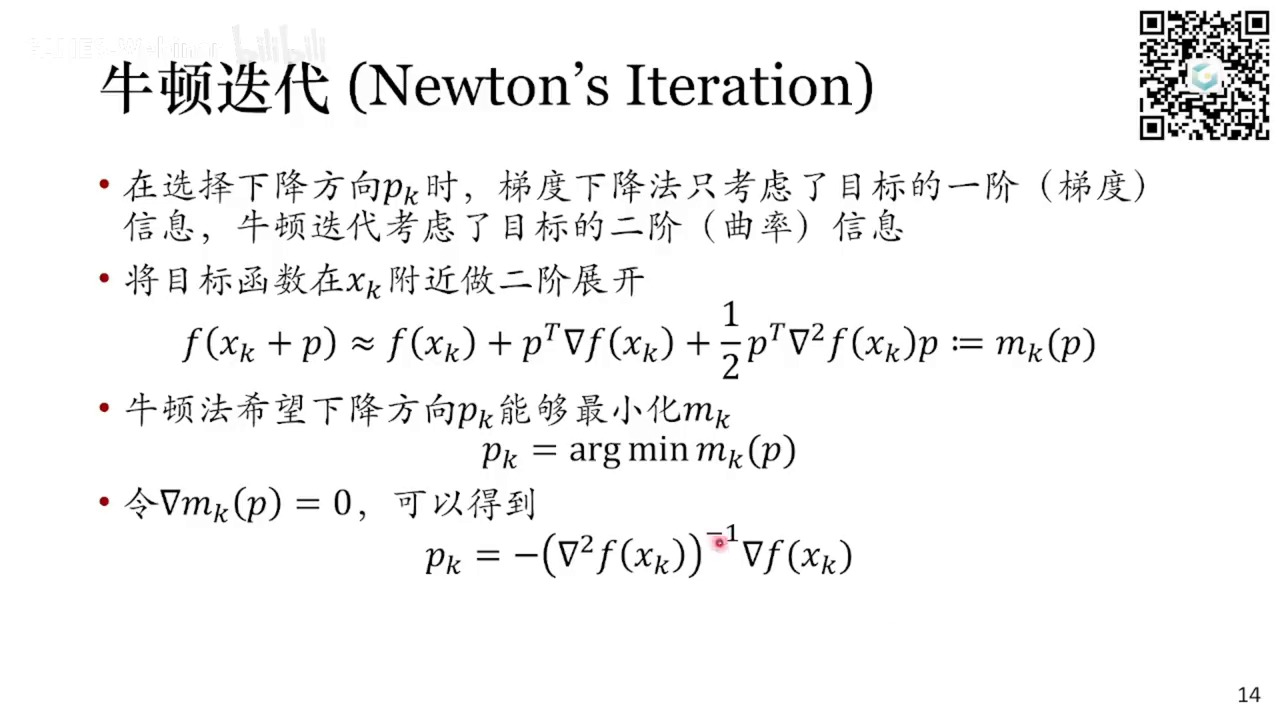
\includegraphics[width=0.92\textwidth]{figures/fig_15_newton1.jpg}
\caption{牛顿迭代：利用目标的二阶展开\vtag}
\end{figure}
\srcnote{00:24:00--00:24:15}
\end{minipage}


梯度下降在选择下降方向时只考虑了目标的一阶（梯度）信息。讲者问：有没有可能使用函数局部的二阶信息，也就是曲率信息，来获得更快的收敛速度？这就是牛顿迭代（Newton's iteration）。将目标函数在 $x_k$ 附近做二阶展开：
\begin{equation}
f(x_k+p)\approx f(x_k)+p^{\mathrm T}\nabla f(x_k)+\frac{1}{2}p^{\mathrm T}\nabla^2f(x_k)p:=m_k(p).
\end{equation}
牛顿法希望下降方向 $p_k$ 能最小化 $m_k$，即 $p_k=\arg\min_p m_k(p)$。令 $\nabla m_k(p)=0$，可以得到
\begin{equation}
p_k=-\left(\nabla^2f(x_k)\right)^{-1}\nabla f(x_k).
\end{equation}
它不再像梯度下降那样直接等于负梯度，而是在前面乘上了二阶导数矩阵的逆。

\subsection{海森矩阵与正定性}

\noindent\begin{minipage}{\textwidth}
\begin{figure}[H]
\centering
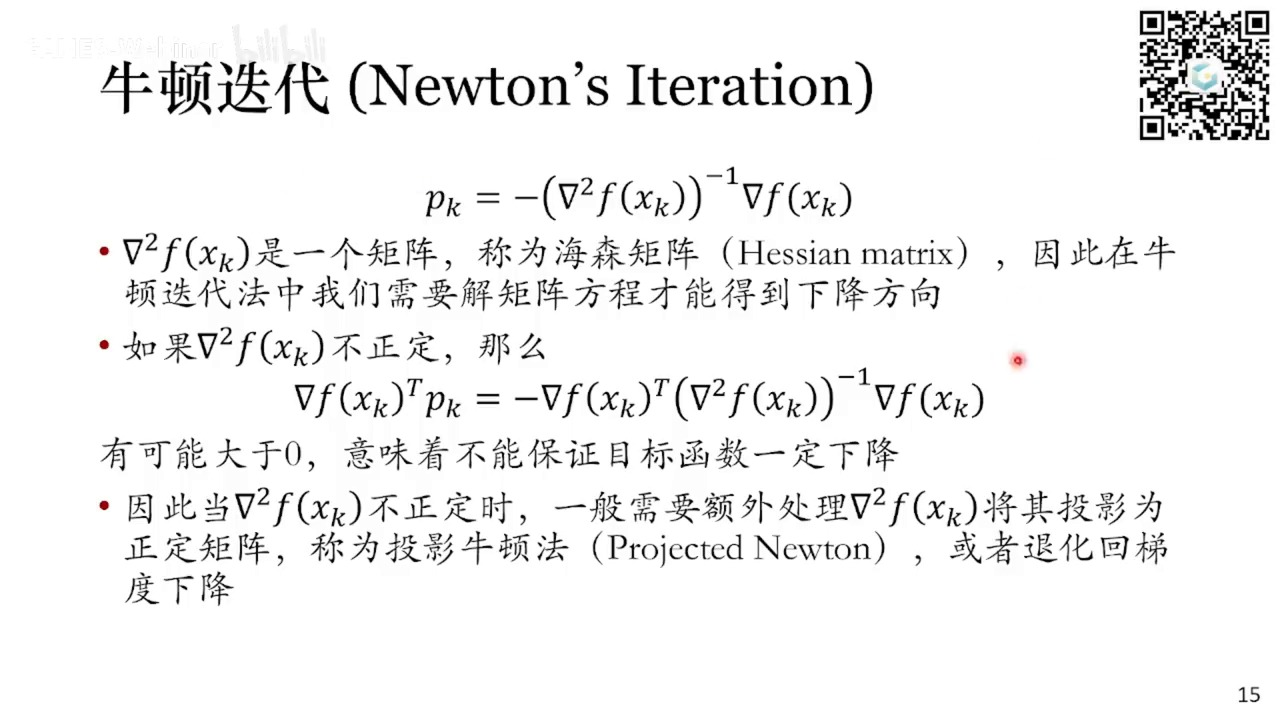
\includegraphics[width=0.92\textwidth]{figures/fig_16_newton2.jpg}
\caption{海森矩阵不正定时的问题与投影牛顿法\vtag}
\end{figure}
\srcnote{00:28:15--00:28:30}
\end{minipage}


$\nabla^2f(x_k)$ 是一个矩阵，称为海森矩阵（Hessian matrix），因此牛顿迭代法中需要解矩阵方程才能得到下降方向。如果 $\nabla^2f(x_k)$ 不正定，那么
\begin{equation}
\nabla f(x_k)^{\mathrm T}p_k=-\nabla f(x_k)^{\mathrm T}\left(\nabla^2f(x_k)\right)^{-1}\nabla f(x_k)
\end{equation}
有可能大于零，意味着沿 $p_k$ 走不能保证目标函数一定下降。讲者解释：这是一个二次型，如果中间的矩阵不正定，梯度方向又恰好对应它某个负特征值的特征向量，整个量就变成正的；而梯度下降相当于中间是单位矩阵，所以总能保证下降。

因此当海森矩阵不正定时，一般需要额外处理，将其投影为正定矩阵，称为投影牛顿法（projected Newton），或者直接退化回梯度下降。

\begin{knowledgebox}{怎样把海森矩阵投影为正定}
讲义作者补充：常见做法是对 $\nabla^2f$ 做特征分解 $Q\Lambda Q^{\mathrm T}$，把负特征值截断为零或一个小正数后再拼回去；在弹性体模拟中，通常对每个单元的局部海森矩阵分别做这种投影再组装，代价远小于对整个大矩阵做分解。另一种简单办法是加上 $\mu I$，并逐步增大 $\mu$ 直到矩阵正定。
\end{knowledgebox}

\noindent\begin{minipage}{\textwidth}
\begin{figure}[H]
\centering
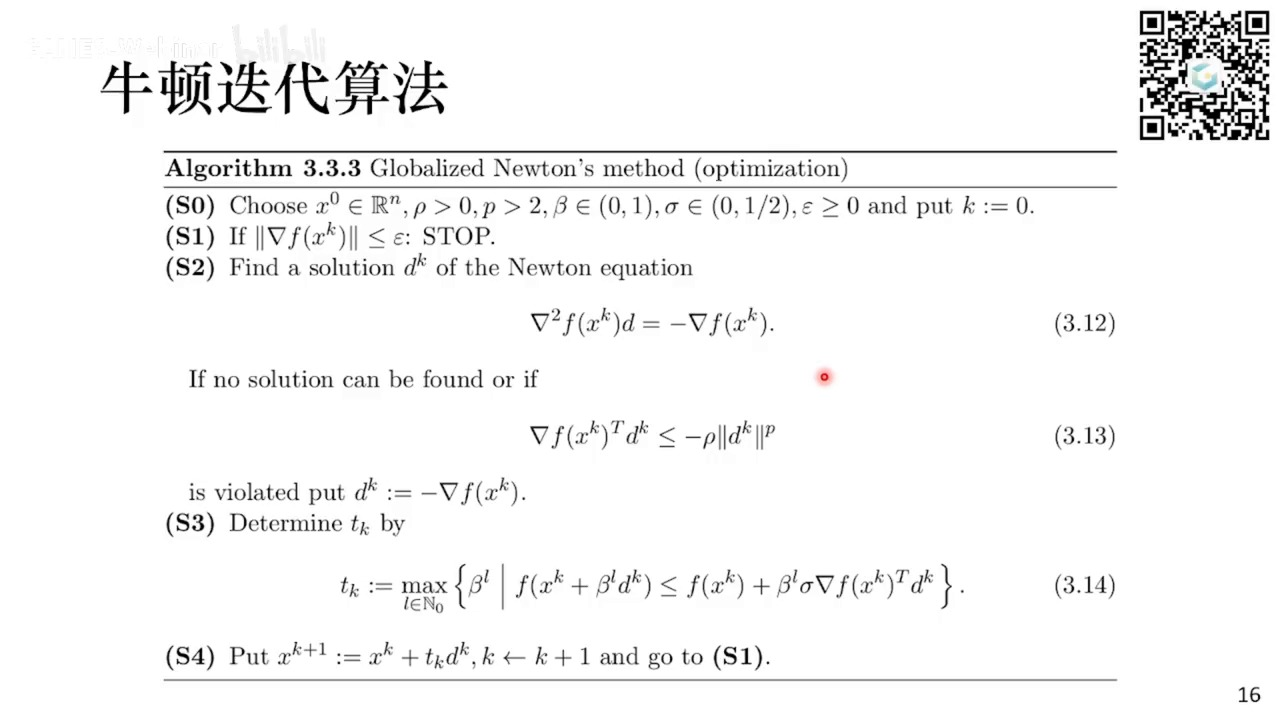
\includegraphics[width=0.92\textwidth]{figures/fig_17_newton_algo.jpg}
\caption{牛顿迭代算法\vtag}
\end{figure}
\srcnote{00:29:15--00:29:30}
\end{minipage}


\subsection{比较}

\noindent\begin{minipage}{\textwidth}
\begin{figure}[H]
\centering
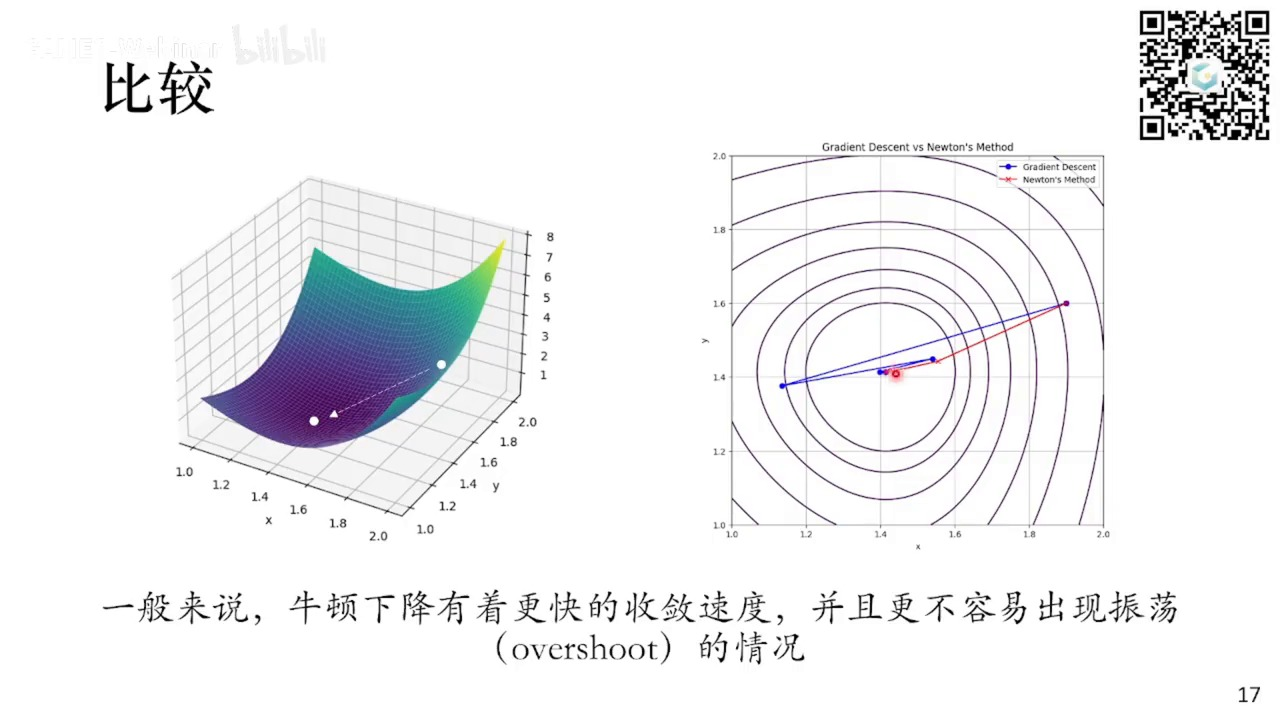
\includegraphics[width=0.92\textwidth]{figures/fig_18_compare.jpg}
\caption{比较：牛顿下降收敛更快，更不容易振荡\vtag}
\end{figure}
\srcnote{00:31:00--00:31:15}
\end{minipage}


讲者用一个二维函数的等高线图比较两种方法。一般来说，牛顿下降有着更快的收敛速度，并且更不容易出现振荡（overshoot）。梯度下降的明显问题是可能出现振荡：虽然每步都满足 Armijo 条件保证函数值下降，但沿梯度方向会在“峡谷”两侧来回跳，像锯齿一样前进。牛顿法利用了二阶信息，收敛快是合理的；与之相应，牛顿法每一步都要解一个矩阵方程来得到下降方向。

\begin{warningbox}{收敛快不等于总时间短}
讲义作者提醒：牛顿法每次迭代要组装并求解一个 $n\times n$ 的线性方程组，而梯度下降只需要一次梯度计算。迭代次数少不代表总耗时少，问题规模很大时，求解海森矩阵方程可能成为瓶颈，这正是下面拟牛顿法的出发点。
\end{warningbox}

\section{拟牛顿法}

\noindent\begin{minipage}{\textwidth}
\begin{figure}[H]
\centering
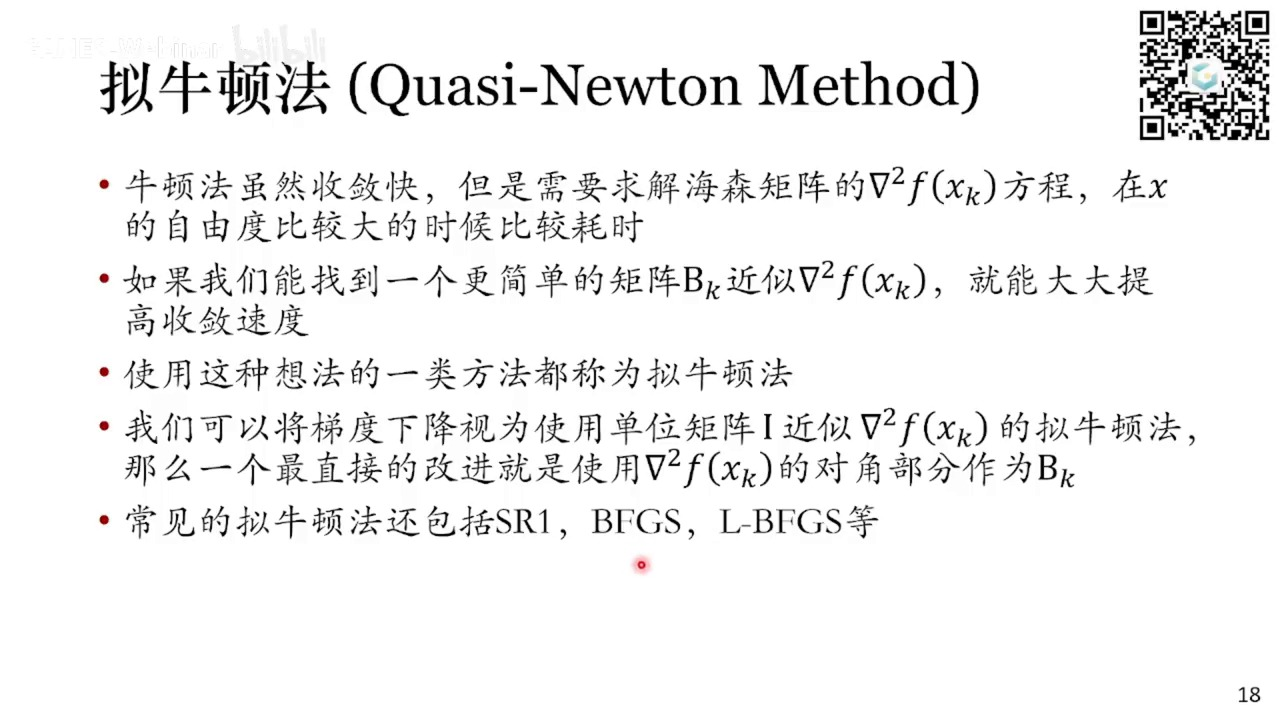
\includegraphics[width=0.92\textwidth]{figures/fig_19_quasi.jpg}
\caption{拟牛顿法：用更简单的矩阵近似海森矩阵\vtag}
\end{figure}
\srcnote{00:34:15--00:34:30}
\end{minipage}


牛顿法虽然收敛快，但需要求解海森矩阵 $\nabla^2f(x_k)$ 的方程，在 $x$ 的自由度比较大的时候比较耗时。如果能找到一个更简单的矩阵 $\mathbf B_k$ 近似 $\nabla^2f(x_k)$，用它代替海森矩阵求下降方向，像牛顿法一样迭代，就能大大提高收敛速度。使用这种想法的一类方法都称为拟牛顿法（quasi-Newton method）。

讲者指出，可以把梯度下降视为使用单位矩阵 $\mathbf I$ 近似海森矩阵的拟牛顿法：直接把单位矩阵的逆乘在梯度前面，相当于直接把负梯度作为下降方向。单位矩阵虽然近似得很粗糙，但它一定正定。一个最直接的改进是使用海森矩阵的对角部分作为 $\mathbf B_k$。常见的拟牛顿法还包括 SR1、BFGS、L-BFGS 等。

\subsection{BFGS 的思想}

\noindent\begin{minipage}{\textwidth}
\begin{figure}[H]
\centering
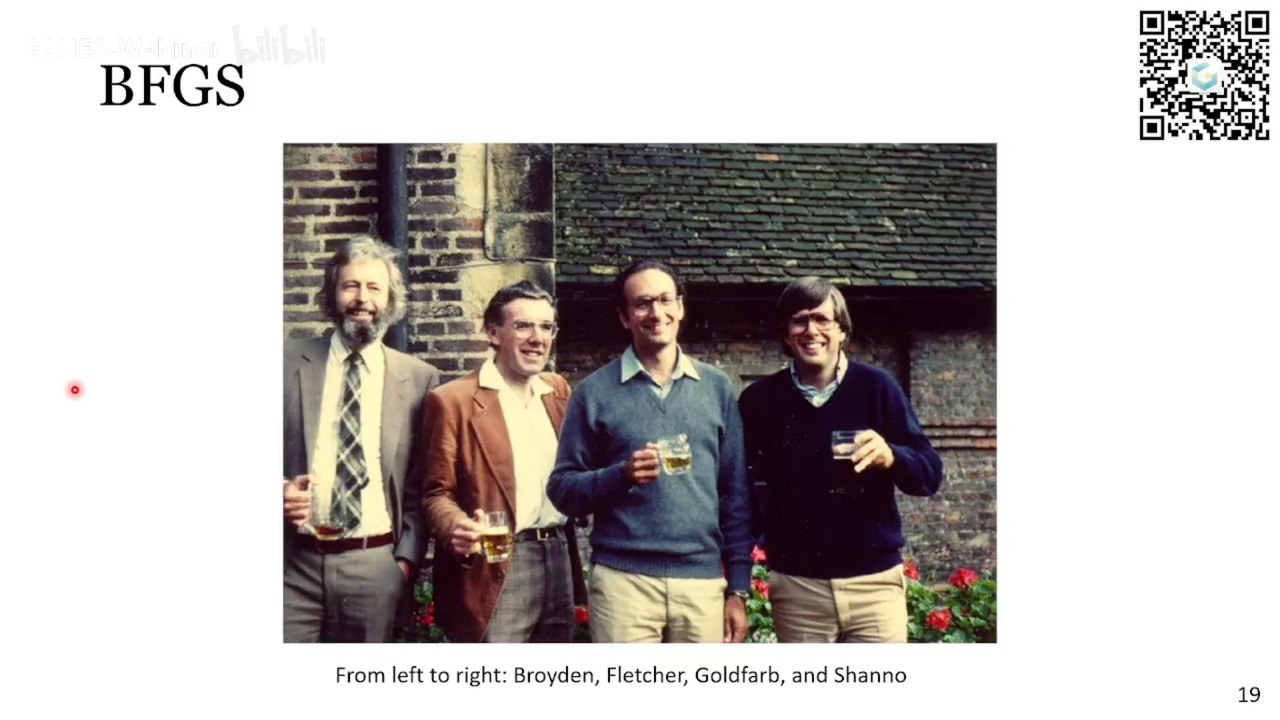
\includegraphics[width=0.92\textwidth]{figures/fig_20_bfgs_people.jpg}
\caption{BFGS 的四位提出者：Broyden、Fletcher、Goldfarb 与 Shanno\vtag}
\end{figure}
\srcnote{00:34:45--00:35:00}
\end{minipage}


讲者重点介绍 BFGS 算法，它是现在非常通用的方法，大家使用各种工业软件或数值求解库时，经常会遇到它。名字来自四位提出者 Broyden、Fletcher、Goldfarb 与 Shanno。

\noindent\begin{minipage}{\textwidth}
\begin{figure}[H]
\centering
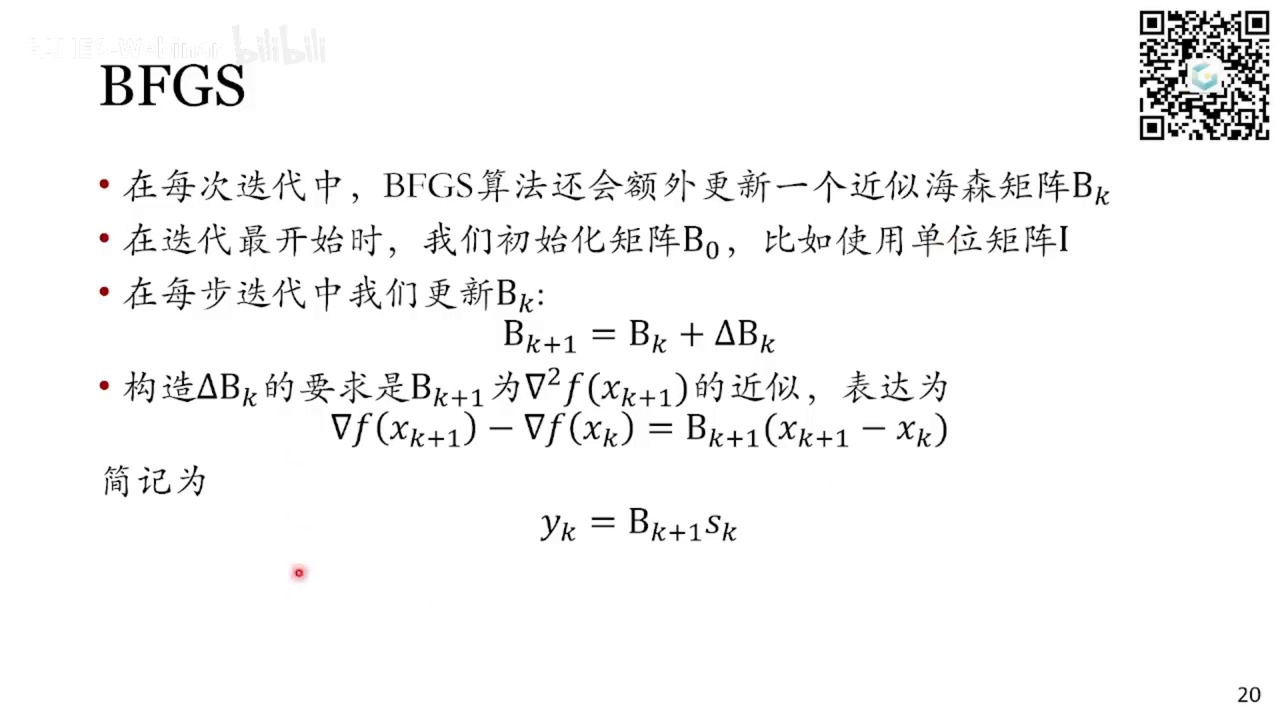
\includegraphics[width=0.92\textwidth]{figures/fig_21_bfgs1.jpg}
\caption{BFGS：维护近似海森矩阵并满足割线条件\vtag}
\end{figure}
\srcnote{00:38:00--00:38:15}
\end{minipage}


在每次迭代中，BFGS 算法会额外更新一个近似海森矩阵 $\mathbf B_k$。迭代最开始时初始化 $\mathbf B_0$，比如使用单位矩阵 $\mathbf I$；每步更新
\begin{equation}
\mathbf B_{k+1}=\mathbf B_k+\Delta\mathbf B_k .
\end{equation}
构造 $\Delta\mathbf B_k$ 的要求是 $\mathbf B_{k+1}$ 为 $\nabla^2f(x_{k+1})$ 的近似。讲者解释：把 $\nabla f$ 在 $x_{k+1}$ 附近展开，梯度之差应约等于海森矩阵乘以位置之差，于是要求
\begin{equation}
\nabla f(x_{k+1})-\nabla f(x_k)=\mathbf B_{k+1}(x_{k+1}-x_k),
\end{equation}
简记为 $y_k=\mathbf B_{k+1}s_k$，其中 $s_k=x_{k+1}-x_k$，$y_k$ 是两点处的梯度差。只要 $\Delta\mathbf B_k$ 满足这个关系，就近似认为 $\mathbf B_{k+1}$ 是海森矩阵的近似。

\subsection{秩为二的更新}

\noindent\begin{minipage}{\textwidth}
\begin{figure}[H]
\centering
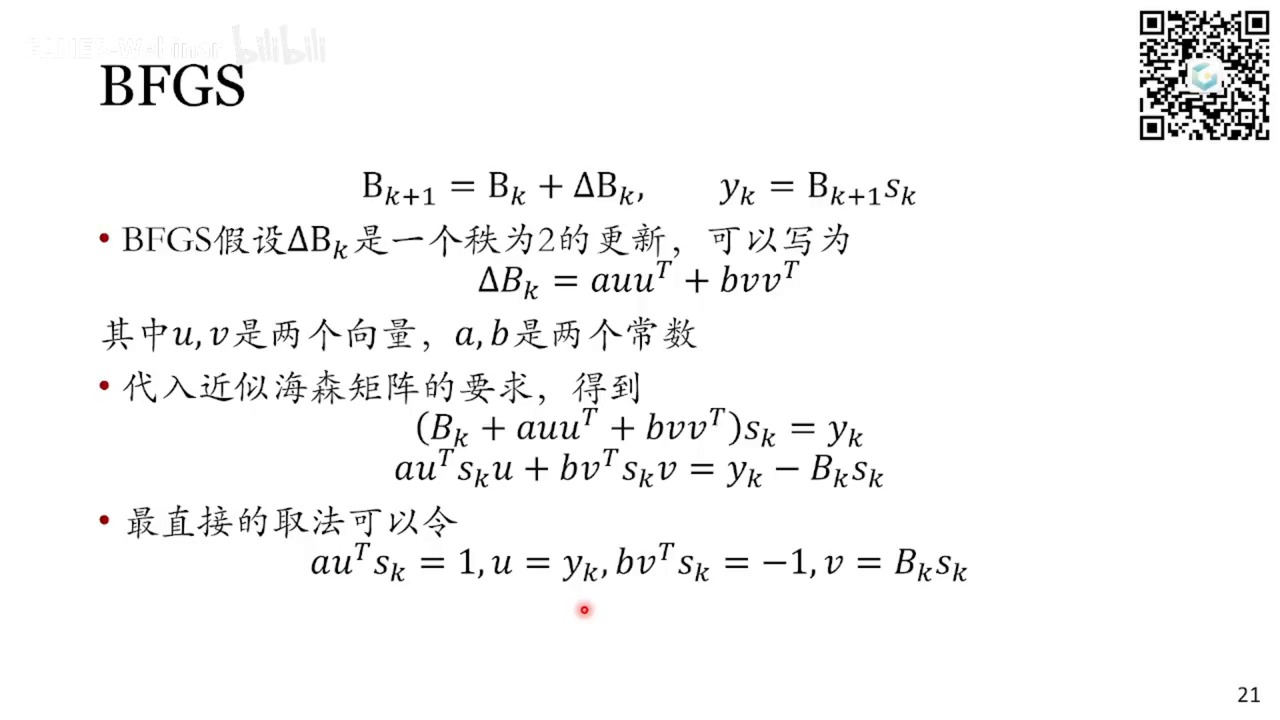
\includegraphics[width=0.92\textwidth]{figures/fig_22_bfgs2.jpg}
\caption{BFGS 假设更新是秩为二的矩阵\vtag}
\end{figure}
\srcnote{00:40:15--00:40:30}
\end{minipage}


BFGS 假设 $\Delta\mathbf B_k$ 是一个秩为 2 的更新，可以写为
\begin{equation}
\Delta\mathbf B_k=a\,uu^{\mathrm T}+b\,vv^{\mathrm T},
\end{equation}
其中 $u,v$ 是两个向量，$a,b$ 是两个常数。代入近似海森矩阵的要求，挪一挪项，得到
\begin{equation}
a\,(u^{\mathrm T}s_k)\,u+b\,(v^{\mathrm T}s_k)\,v=y_k-\mathbf B_ks_k .
\end{equation}
等式右边是已知的。最直接的取法是让左右两项分别对应：
\begin{equation}
a\,u^{\mathrm T}s_k=1,\quad u=y_k,\qquad b\,v^{\mathrm T}s_k=-1,\quad v=\mathbf B_ks_k .
\end{equation}

\noindent\begin{minipage}{\textwidth}
\begin{figure}[H]
\centering
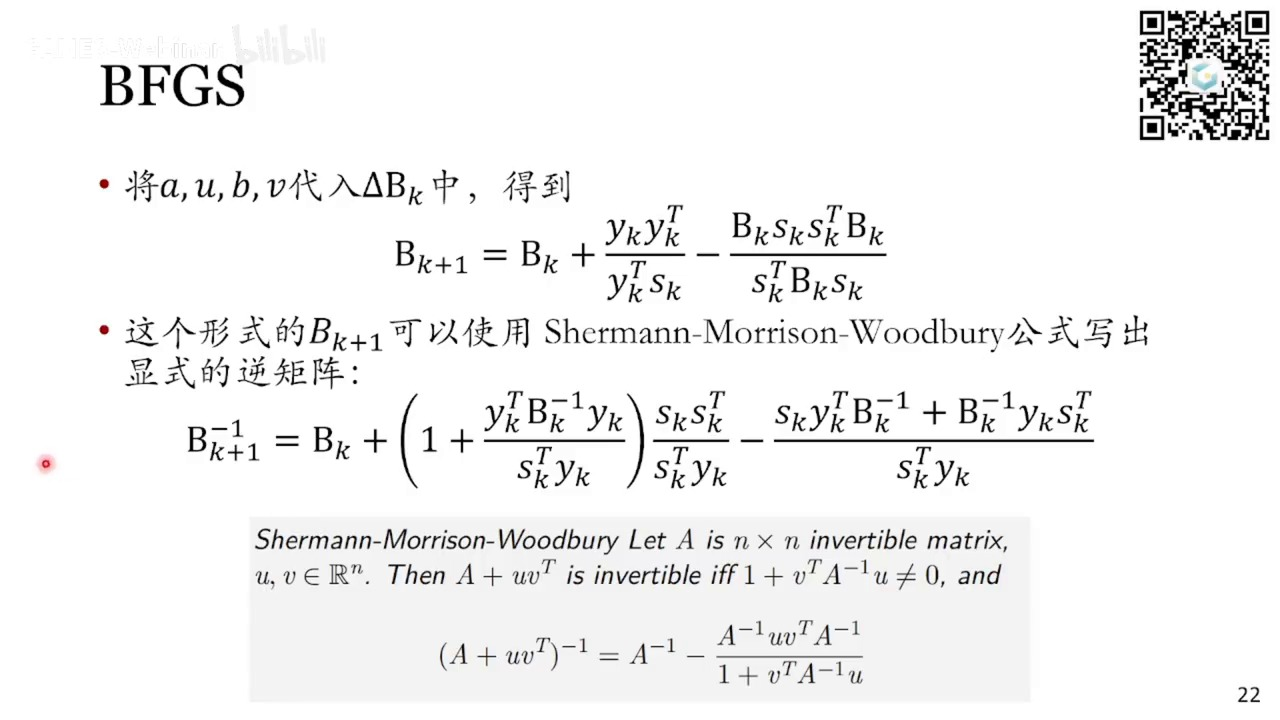
\includegraphics[width=0.92\textwidth]{figures/fig_23_bfgs3.jpg}
\caption{BFGS 的更新公式与逆矩阵的显式形式\vtag}
\end{figure}
\srcnote{00:41:45--00:42:00}
\end{minipage}


将 $a,u,b,v$ 代入 $\Delta\mathbf B_k$ 中，得到
\begin{equation}
\mathbf B_{k+1}=\mathbf B_k+\frac{y_ky_k^{\mathrm T}}{y_k^{\mathrm T}s_k}-\frac{\mathbf B_ks_ks_k^{\mathrm T}\mathbf B_k}{s_k^{\mathrm T}\mathbf B_ks_k}.
\end{equation}
求下降方向需要的是 $\mathbf B_{k+1}^{-1}$。这个形式可以使用 Sherman--Morrison--Woodbury 公式写出显式的逆矩阵：
\begin{equation}
\mathbf B_{k+1}^{-1}=\mathbf B_k^{-1}+\left(1+\frac{y_k^{\mathrm T}\mathbf B_k^{-1}y_k}{s_k^{\mathrm T}y_k}\right)\frac{s_ks_k^{\mathrm T}}{s_k^{\mathrm T}y_k}-\frac{\mathbf B_k^{-1}y_ks_k^{\mathrm T}+s_ky_k^{\mathrm T}\mathbf B_k^{-1}}{s_k^{\mathrm T}y_k}.
\end{equation}
讲者说，因为后面两项都是低秩的，逆矩阵也只需要在 $\mathbf B_k^{-1}$ 上做低秩修正，而不必真的去解矩阵方程。

\begin{knowledgebox}{Sherman--Morrison--Woodbury 公式}
若 $A$ 可逆，$U,V$ 为 $n\times k$ 矩阵，则 $(A+UV^{\mathrm T})^{-1}=A^{-1}-A^{-1}U(I+V^{\mathrm T}A^{-1}U)^{-1}V^{\mathrm T}A^{-1}$。当 $k$ 很小时，右边只需要求一个 $k\times k$ 小矩阵的逆。BFGS 的更新是秩为 2 的修正，所以求逆的代价只相当于做几次向量运算。
\end{knowledgebox}

\subsection{正定性}

\noindent\begin{minipage}{\textwidth}
\begin{figure}[H]
\centering
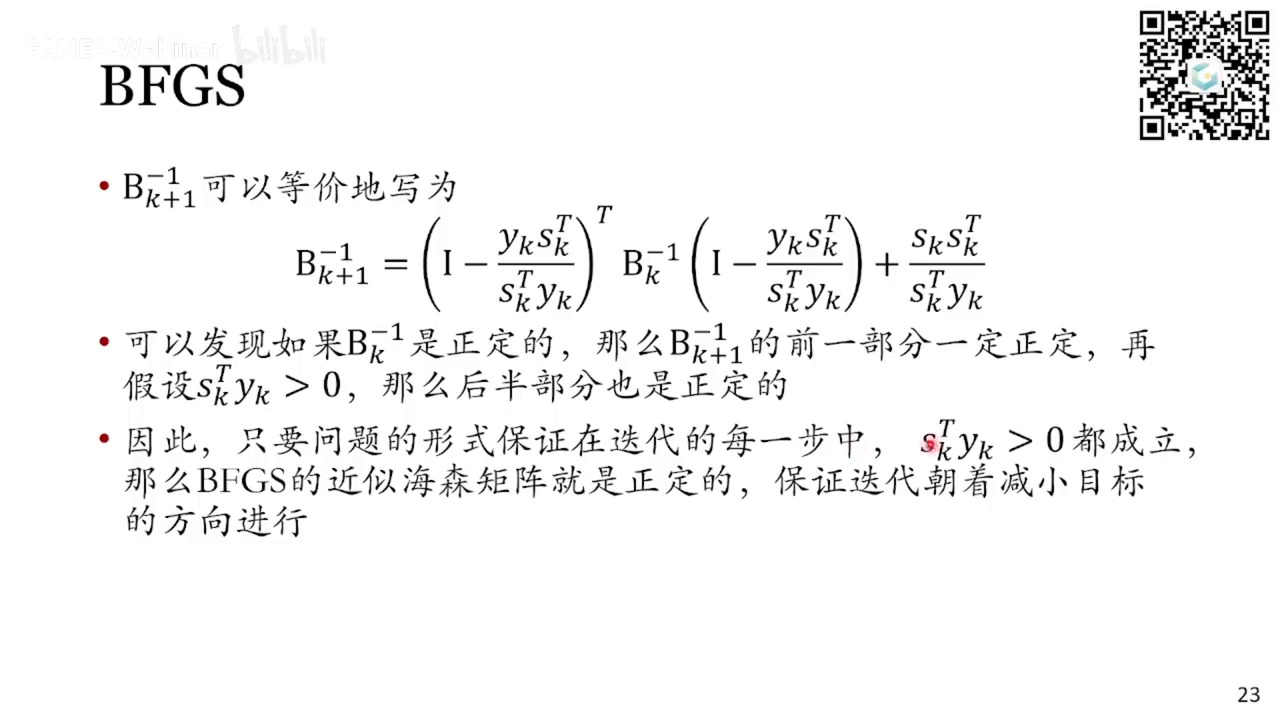
\includegraphics[width=0.92\textwidth]{figures/fig_24_bfgs4.jpg}
\caption{BFGS 的逆矩阵的等价形式与正定性\vtag}
\end{figure}
\srcnote{00:44:00--00:44:15}
\end{minipage}


$\mathbf B_{k+1}^{-1}$ 可以等价地写为
\begin{equation}
\mathbf B_{k+1}^{-1}=\left(\mathbf I-\frac{s_ky_k^{\mathrm T}}{s_k^{\mathrm T}y_k}\right)\mathbf B_k^{-1}\left(\mathbf I-\frac{y_ks_k^{\mathrm T}}{s_k^{\mathrm T}y_k}\right)+\frac{s_ks_k^{\mathrm T}}{s_k^{\mathrm T}y_k}.
\end{equation}
讲者说大家可以自己检查它与上一式等价。改写之后可以发现：如果 $\mathbf B_k^{-1}$ 是正定的，那么前一部分一定半正定；再假设 $s_k^{\mathrm T}y_k>0$，那么后一部分也是半正定的，两者相加正定。因此，只要问题的形式保证在迭代的每一步中 $s_k^{\mathrm T}y_k>0$ 都成立，BFGS 的近似海森矩阵就是正定的，保证迭代朝着减小目标的方向进行。这就回答了牛顿法中海森矩阵不正定的担忧。

\begin{importantbox}{$s_k^{\mathrm T}y_k>0$ 从哪里来}
$s_k$ 是位置之差，$y_k$ 是梯度之差。讲者说这个条件是否一直成立由问题的具体形式来保证：如果目标函数是凸的，梯度差与位置差的内积总是非负。讲义作者补充：对非凸问题，一般在线搜索中要求满足比 Armijo 更强的 Wolfe 曲率条件，它能保证 $s_k^{\mathrm T}y_k>0$。
\end{importantbox}

\noindent\begin{minipage}{\textwidth}
\begin{figure}[H]
\centering
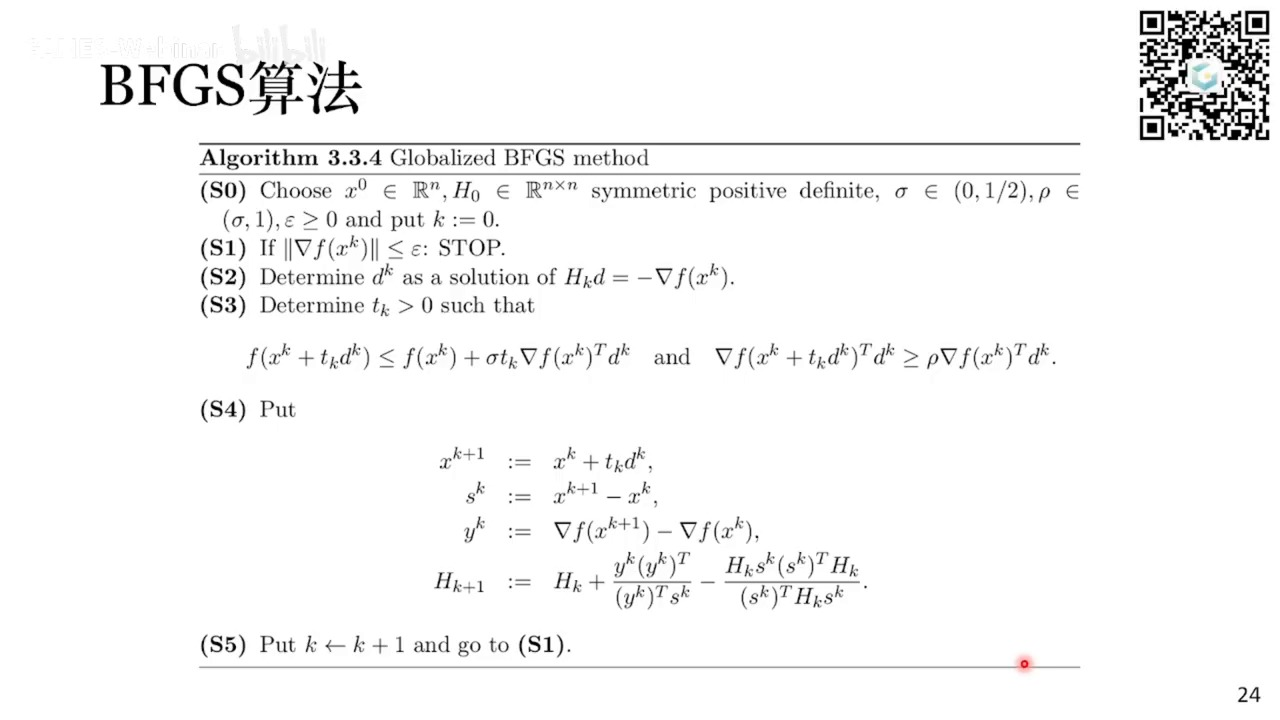
\includegraphics[width=0.92\textwidth]{figures/fig_25_bfgs_algo.jpg}
\caption{BFGS 算法\vtag}
\end{figure}
\srcnote{00:45:30--00:45:45}
\end{minipage}


整个 BFGS 算法里，下降方向和牛顿法一样由矩阵方程给出，但矩阵是由 BFGS 迭代更新的近似海森矩阵；由于它的逆可以显式更新，实际上只需要矩阵乘向量。

\subsection{L-BFGS}

\noindent\begin{minipage}{\textwidth}
\begin{figure}[H]
\centering
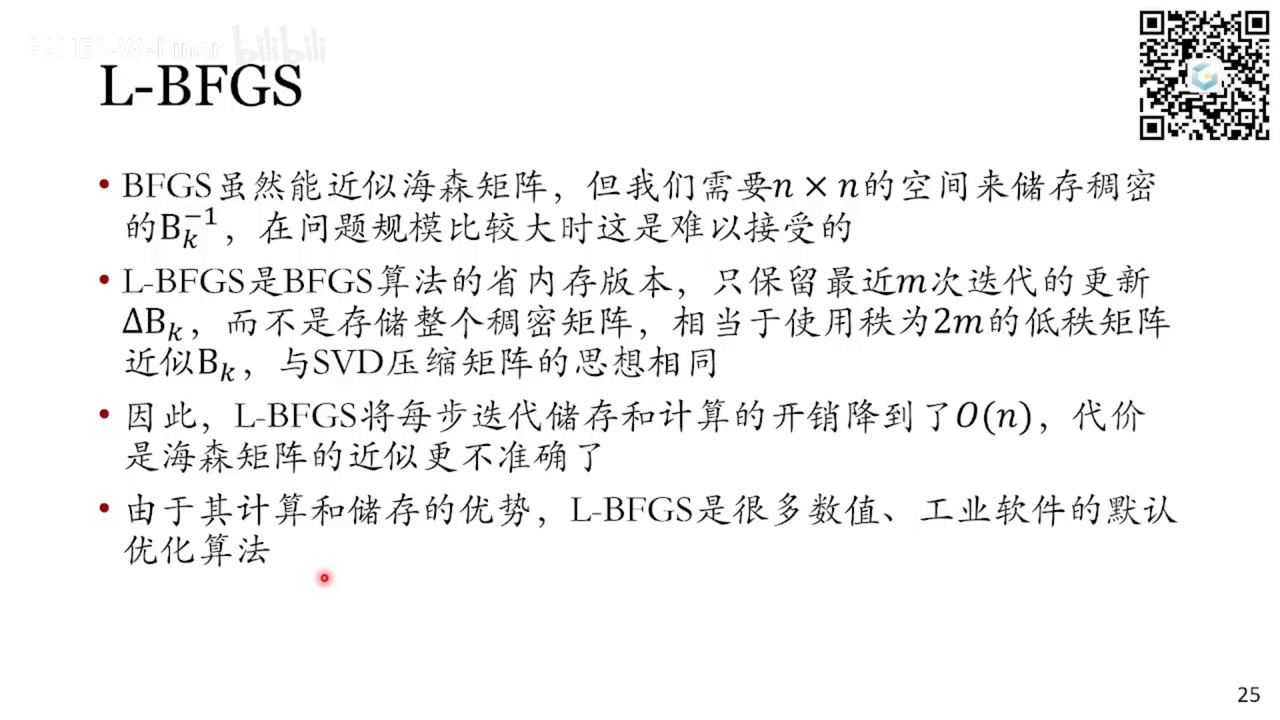
\includegraphics[width=0.92\textwidth]{figures/fig_26_lbfgs.jpg}
\caption{L-BFGS：只保留最近若干次更新的省内存版本\vtag}
\end{figure}
\srcnote{00:48:45--00:49:00}
\end{minipage}


BFGS 虽然能近似海森矩阵，但需要 $n\times n$ 的空间来储存稠密的 $\mathbf B_k^{-1}$。讲者举例，如果像上一讲那样网格有几百万个节点，$n\times n$ 就是很大很大的空间，这在问题规模比较大时难以接受。

L-BFGS 是 BFGS 的省内存版本，只保留最近 $m$ 次迭代的更新 $\Delta\mathbf B_k$，而不是存储整个稠密矩阵，相当于使用秩为 $2m$ 的低秩矩阵近似 $\mathbf B_k$，只需要存 $2m$ 个向量。这与用 SVD 压缩矩阵的思想相同。因此 L-BFGS 将每步迭代储存和计算的开销降到了 $O(n)$，代价是海森矩阵的近似更不准确了。由于其计算和储存上的优势，L-BFGS 是很多数值、工业软件的默认优化算法。

\begin{knowledgebox}{L-BFGS 的双循环递归}
讲义作者补充：实际实现中并不显式构造矩阵，而是用两次长度为 $m$ 的循环，直接由最近的 $(s_i,y_i)$ 对把梯度变换成下降方向 $-\mathbf B_k^{-1}\nabla f$。每次只需要若干内积和向量加法，$m$ 通常取 $5$ 到 $20$ 左右。
\end{knowledgebox}

\subsection{不动点迭代也是拟牛顿法}

\noindent\begin{minipage}{\textwidth}
\begin{figure}[H]
\centering
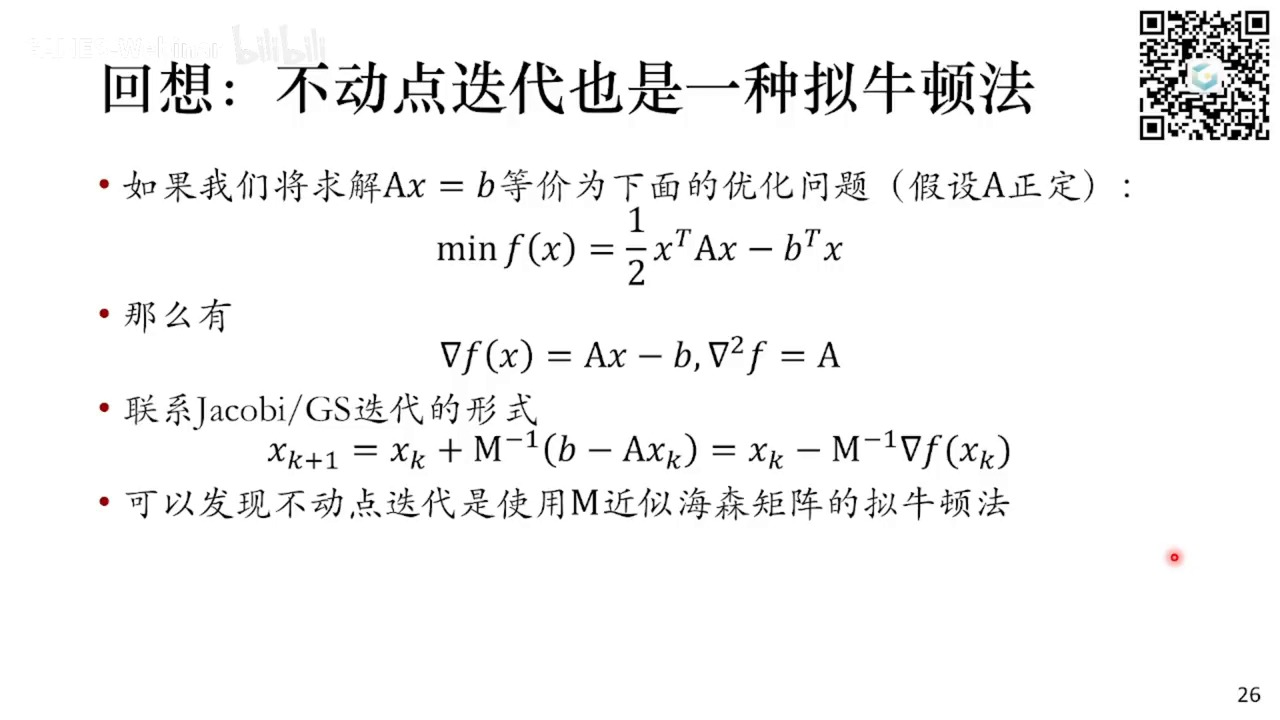
\includegraphics[width=0.92\textwidth]{figures/fig_27_fixed_point.jpg}
\caption{回想：不动点迭代也是一种拟牛顿法\vtag}
\end{figure}
\srcnote{00:50:45--00:51:00}
\end{minipage}


讲者回顾上一讲介绍的用不动点迭代求解矩阵方程。如果把求解 $\mathbf Ax=b$ 等价为下面的优化问题（假设 $\mathbf A$ 正定）：
\begin{equation}
\min f(x)=\frac{1}{2}x^{\mathrm T}\mathbf Ax-b^{\mathrm T}x,
\end{equation}
那么有 $\nabla f(x)=\mathbf Ax-b$，$\nabla^2f=\mathbf A$。联系 Jacobi 或 Gauss--Seidel 迭代的形式
\begin{equation}
x_{k+1}=x_k+\mathbf M^{-1}(b-\mathbf Ax_k)=x_k-\mathbf M^{-1}\nabla f(x_k),
\end{equation}
可以发现不动点迭代是使用 $\mathbf M$ 近似海森矩阵 $\mathbf A$ 的拟牛顿法：Jacobi 用的是对角部分，Gauss--Seidel 用的是下三角部分。

讲者小结第一部分：无约束优化里比较核心的几种方法是梯度下降法、牛顿法以及拟牛顿法，其中要特别注意 BFGS 和 L-BFGS 算法。

\section{带约束优化}

\noindent\begin{minipage}{\textwidth}
\begin{figure}[H]
\centering
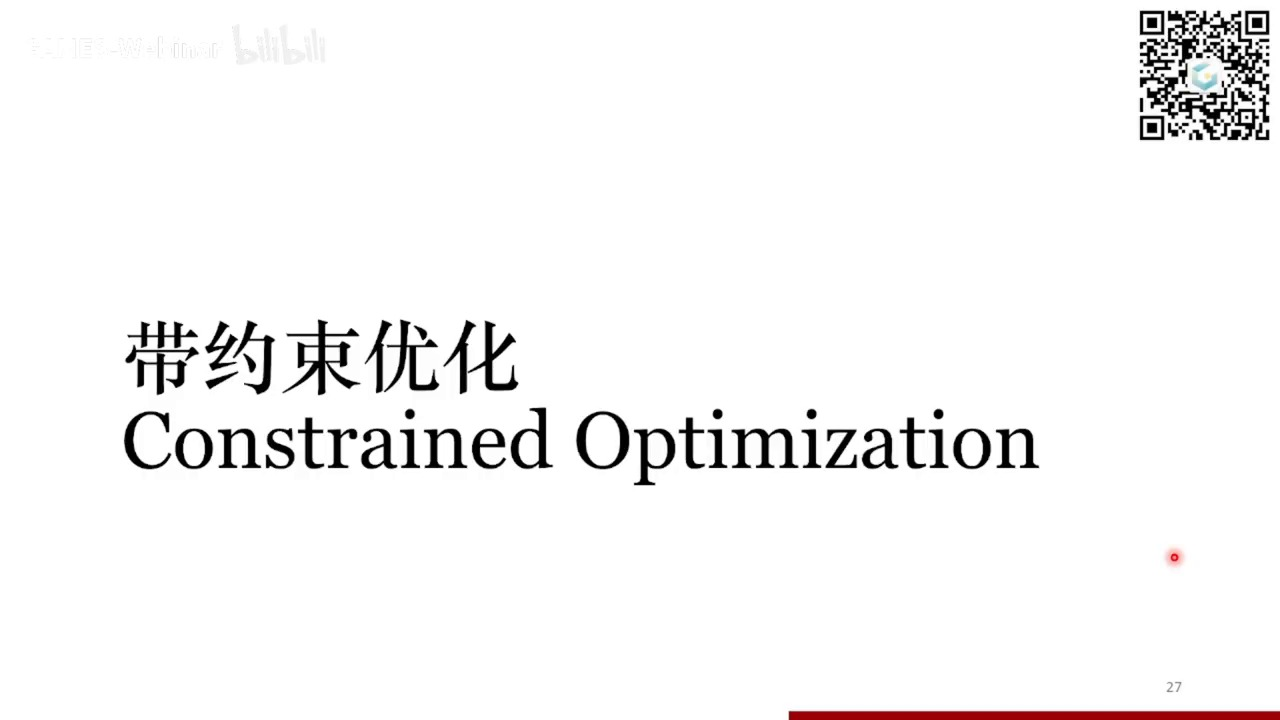
\includegraphics[width=0.92\textwidth]{figures/fig_28_constrained_title.jpg}
\caption{第二部分：带约束优化\vtag}
\end{figure}
\srcnote{00:51:15--00:51:30}
\end{minipage}


\noindent\begin{minipage}{\textwidth}
\begin{figure}[H]
\centering
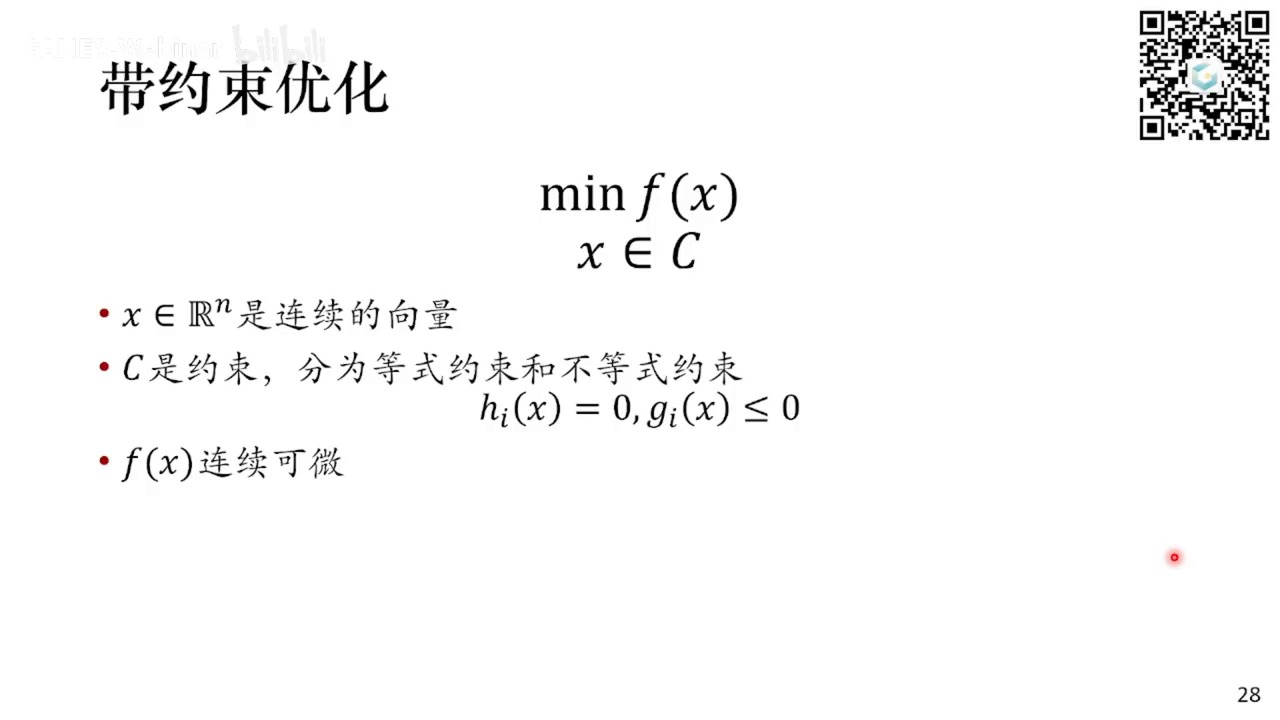
\includegraphics[width=0.92\textwidth]{figures/fig_29_constrained.jpg}
\caption{带约束优化：等式约束与不等式约束\vtag}
\end{figure}
\srcnote{00:51:30--00:51:45}
\end{minipage}


带约束的优化问题写为
\begin{equation}
\min_{x\in C}f(x),\qquad C:\ h_i(x)=0,\quad g_i(x)\le 0 ,
\end{equation}
其中 $x\in\mathbb R^n$ 是连续的向量，约束分为等式约束和不等式约束，$f(x)$ 连续可微。

\noindent\begin{minipage}{\textwidth}
\begin{figure}[H]
\centering
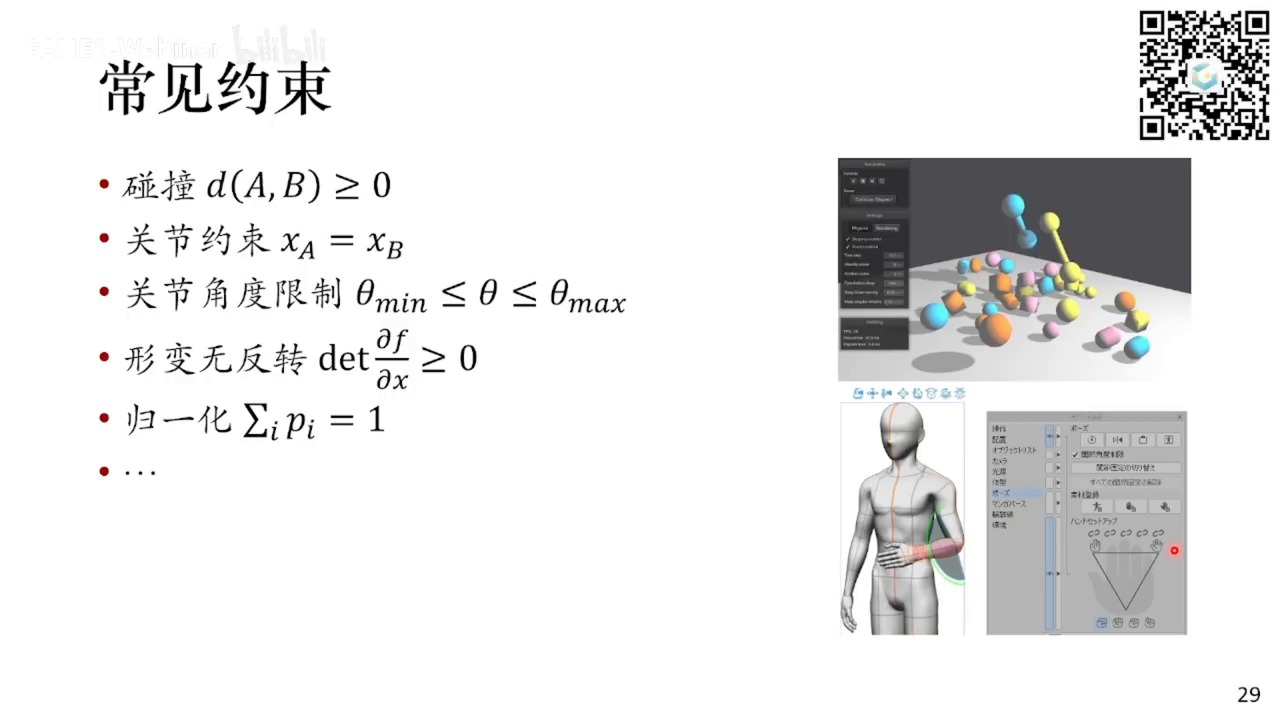
\includegraphics[width=0.92\textwidth]{figures/fig_30_common_constraints.jpg}
\caption{图形学中常见的约束\vtag}
\end{figure}
\srcnote{00:52:30--00:52:45}
\end{minipage}


图形学中常见的约束有：
\begin{itemize}
\item 碰撞：两个物体之间的距离 $d(A,B)\ge 0$；
\item 关节约束：比如人手上的关节，两个部分在关节处的位置应该一样，$x_A=x_B$；
\item 关节角度限制：$\theta_{\min}\le\theta\le\theta_{\max}$，讲者说关节不能弯得过度；
\item 形变无反转：$\det\frac{\partial f}{\partial x}\ge 0$；
\item 归一化：$\sum_ip_i=1$。
\end{itemize}

\section{等式约束与拉格朗日乘子}

\subsection{最优条件}

\noindent\begin{minipage}{\textwidth}
\begin{figure}[H]
\centering
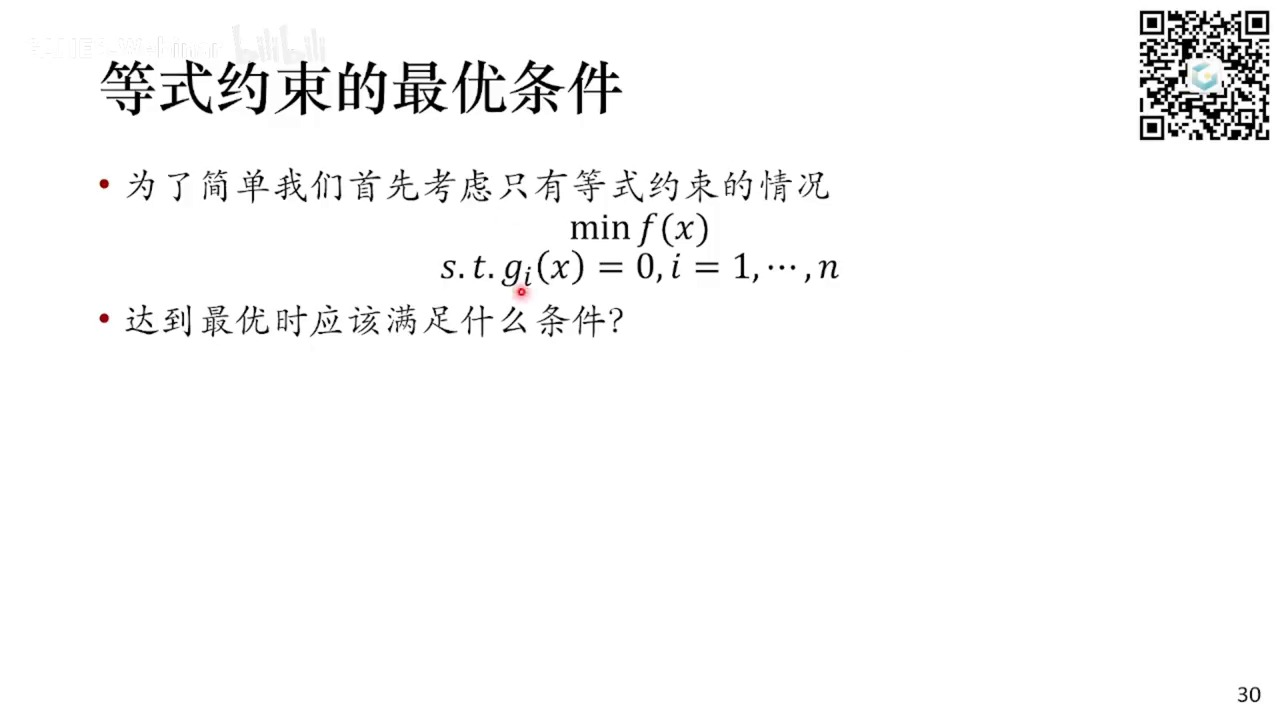
\includegraphics[width=0.92\textwidth]{figures/fig_31_eq_opt1.jpg}
\caption{等式约束的最优条件：达到最优时应满足什么\vtag}
\end{figure}
\srcnote{00:53:00--00:53:15}
\end{minipage}


为了简单，首先考虑只有等式约束的情况：
\begin{equation}
\min f(x)\quad\mathrm{s.t.}\quad g_i(x)=0,\ i=1,\dots,n .
\end{equation}
要回答的第一个问题是：达到最优时应该满足什么条件？

\noindent\begin{minipage}{\textwidth}
\begin{figure}[H]
\centering
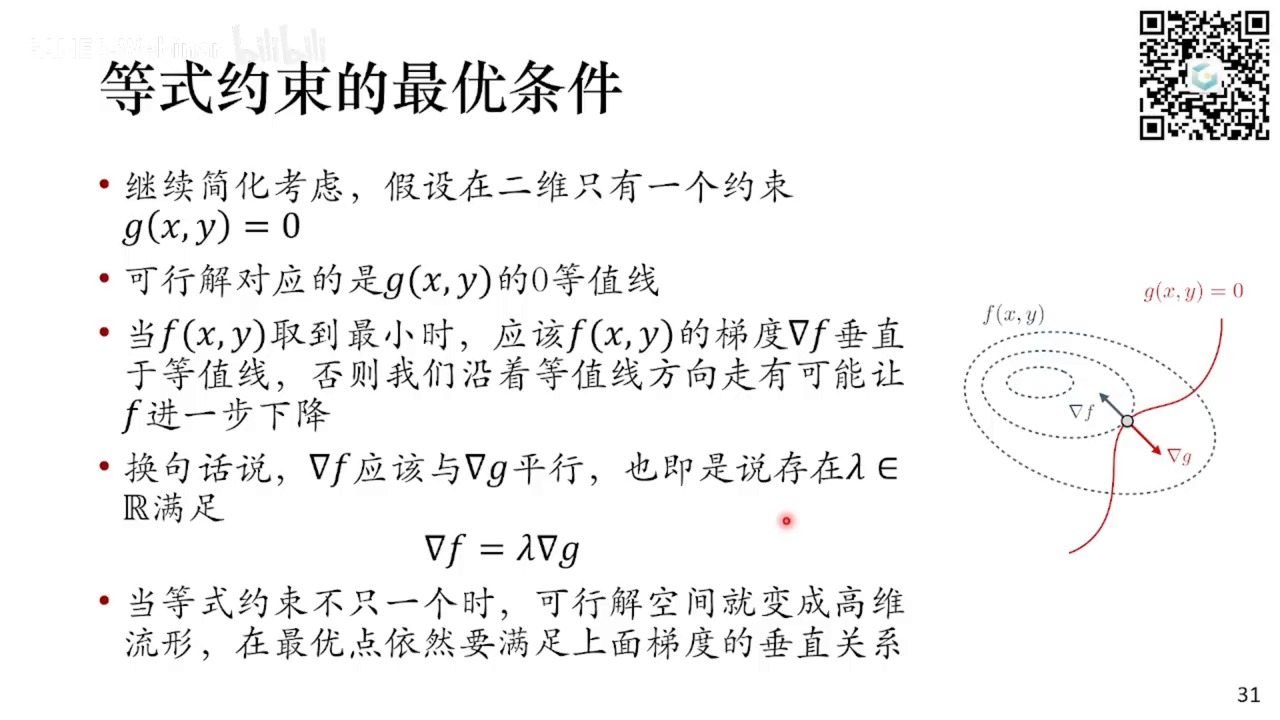
\includegraphics[width=0.92\textwidth]{figures/fig_32_eq_opt2.jpg}
\caption{二维情形：$\nabla f$ 应与约束曲线垂直\vtag}
\end{figure}
\srcnote{00:55:30--00:55:45}
\end{minipage}


继续简化，假设在二维只有一个约束 $g(x,y)=0$。可行解对应的是 $g(x,y)$ 的零等值线。当 $f(x,y)$ 取到最小时，$f$ 的梯度 $\nabla f$ 应该垂直于这条等值线。讲者解释：假如在某点上 $\nabla f$ 与曲线不垂直，就意味着沿曲线的某个方向往前走一点，还有可能让 $f$ 继续下降，这个点就不是最优点。换句话说，$\nabla f$ 应该与 $\nabla g$ 平行，也就是存在 $\lambda\in\mathbb R$ 满足
\begin{equation}
\nabla f=\lambda\nabla g .
\end{equation}
当等式约束不只一个时，可行解空间就变成高维流形，在最优点依然要满足梯度的垂直关系。

\noindent\begin{minipage}{\textwidth}
\begin{figure}[H]
\centering
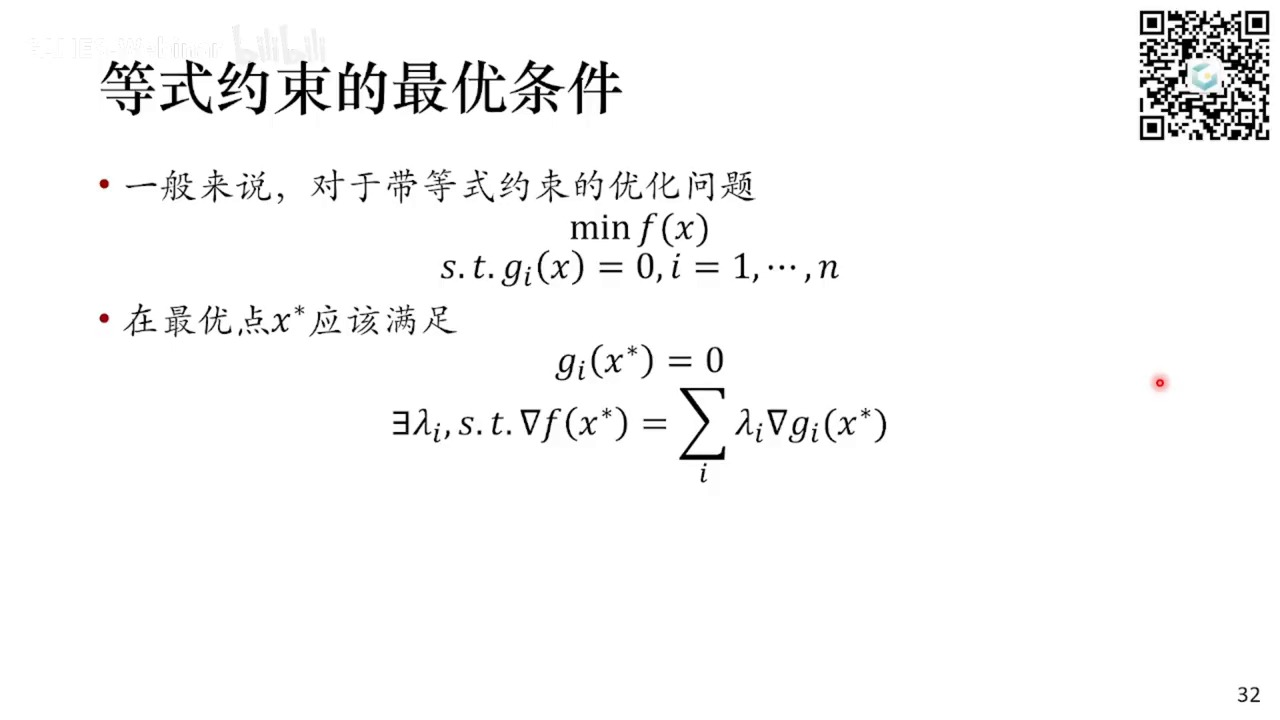
\includegraphics[width=0.92\textwidth]{figures/fig_33_eq_opt3.jpg}
\caption{一般的等式约束最优条件\vtag}
\end{figure}
\srcnote{00:56:30--00:56:45}
\end{minipage}


一般来说，对带等式约束的优化问题，在最优点 $x^*$ 应该满足两条：第一，最优点一定满足所有约束；第二，存在一组 $\lambda_i$，使得 $f$ 的梯度等于约束梯度的线性组合：
\begin{equation}
g_i(x^*)=0,\qquad \exists\lambda_i,\ \mathrm{s.t.}\ \nabla f(x^*)=\sum_i\lambda_i\nabla g_i(x^*).
\end{equation}

\subsection{拉格朗日函数}

\noindent\begin{minipage}{\textwidth}
\begin{figure}[H]
\centering
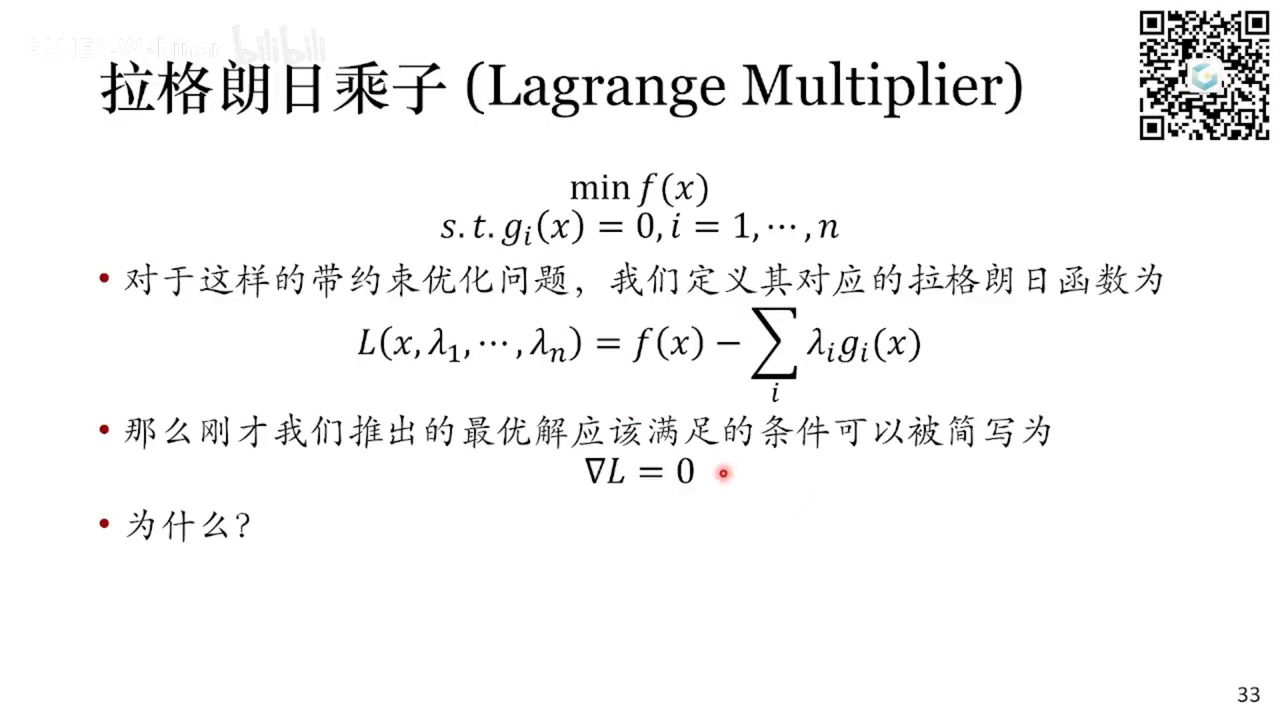
\includegraphics[width=0.92\textwidth]{figures/fig_34_lagrange1.jpg}
\caption{拉格朗日乘子：定义拉格朗日函数\vtag}
\end{figure}
\srcnote{00:57:45--00:58:00}
\end{minipage}


对于这样的带约束优化问题，定义其对应的拉格朗日函数为
\begin{equation}
L(x,\lambda_1,\dots,\lambda_n)=f(x)-\sum_i\lambda_ig_i(x),
\end{equation}
它是 $x$ 以及一组新变量 $\lambda_1,\dots,\lambda_n$ 的函数，$\lambda_i$ 称为拉格朗日乘子。刚才推出的最优条件可以简写为 $\nabla L=0$。为什么？

\noindent\begin{minipage}{\textwidth}
\begin{figure}[H]
\centering
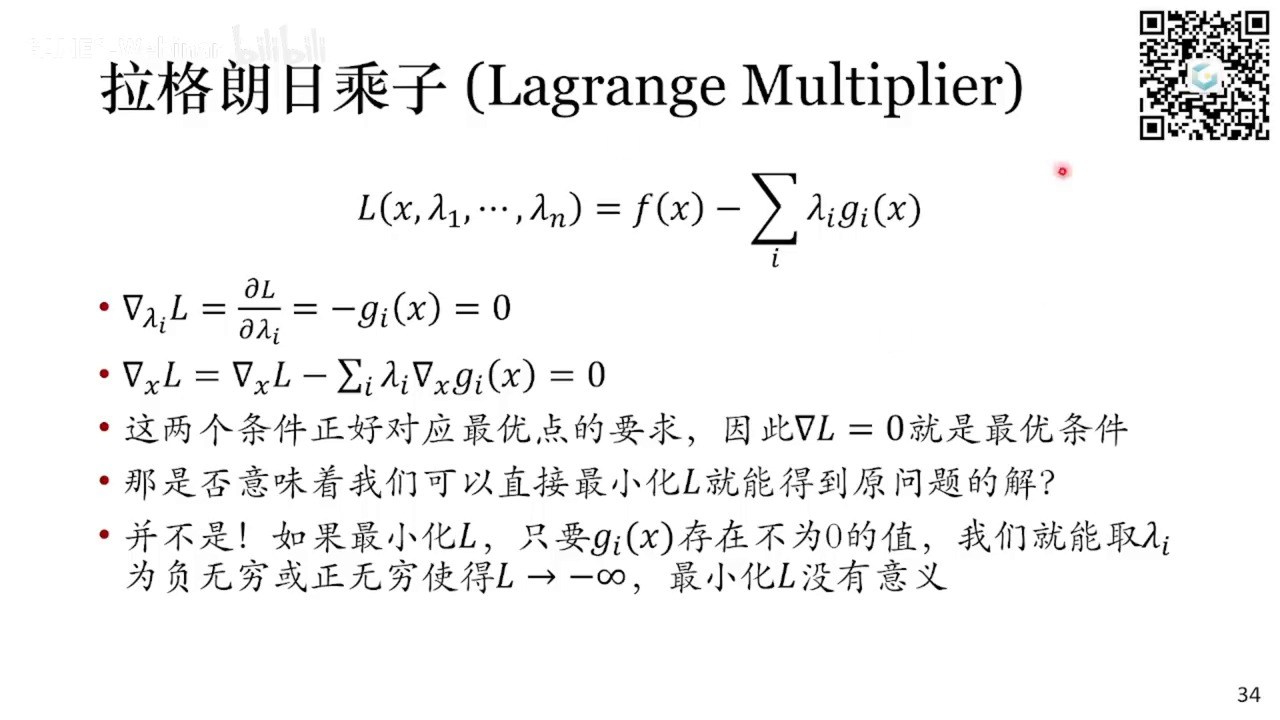
\includegraphics[width=0.92\textwidth]{figures/fig_35_lagrange2.jpg}
\caption{$\nabla L=0$ 就是最优条件，但不能直接最小化 $L$\vtag}
\end{figure}
\srcnote{00:59:45--01:00:00}
\end{minipage}


对 $\lambda_i$ 求导，$\nabla_{\lambda_i}L=\frac{\partial L}{\partial\lambda_i}=-g_i(x)=0$，就是满足约束；对 $x$ 求导，
\begin{equation}
\nabla_xL=\nabla_xf-\sum_i\lambda_i\nabla_xg_i(x)=0,
\end{equation}
就是梯度的平行关系。这两个条件正好对应最优点的要求，因此 $\nabla L=0$ 就是最优条件。

\begin{warningbox}{课件上的一个笔误}
课件第 34 页把 $x$ 方向的条件写成了 $\nabla_xL=\nabla_xL-\sum_i\lambda_i\nabla_xg_i(x)=0$，等号右边第一项应是 $\nabla_xf$ 而不是 $\nabla_xL$，上式已按拉格朗日函数的定义改正。
\end{warningbox}

那是否意味着可以直接最小化 $L$ 就能得到原问题的解？讲者说，并不是！观察拉格朗日函数的形式，如果随便取一个 $x$ 让 $g_i(x)\ne 0$，$\lambda_i$ 就可以取正无穷或负无穷，使得 $L\to-\infty$，所以最小化 $L$ 没有意义。

\subsection{min-max 博弈}

\noindent\begin{minipage}{\textwidth}
\begin{figure}[H]
\centering
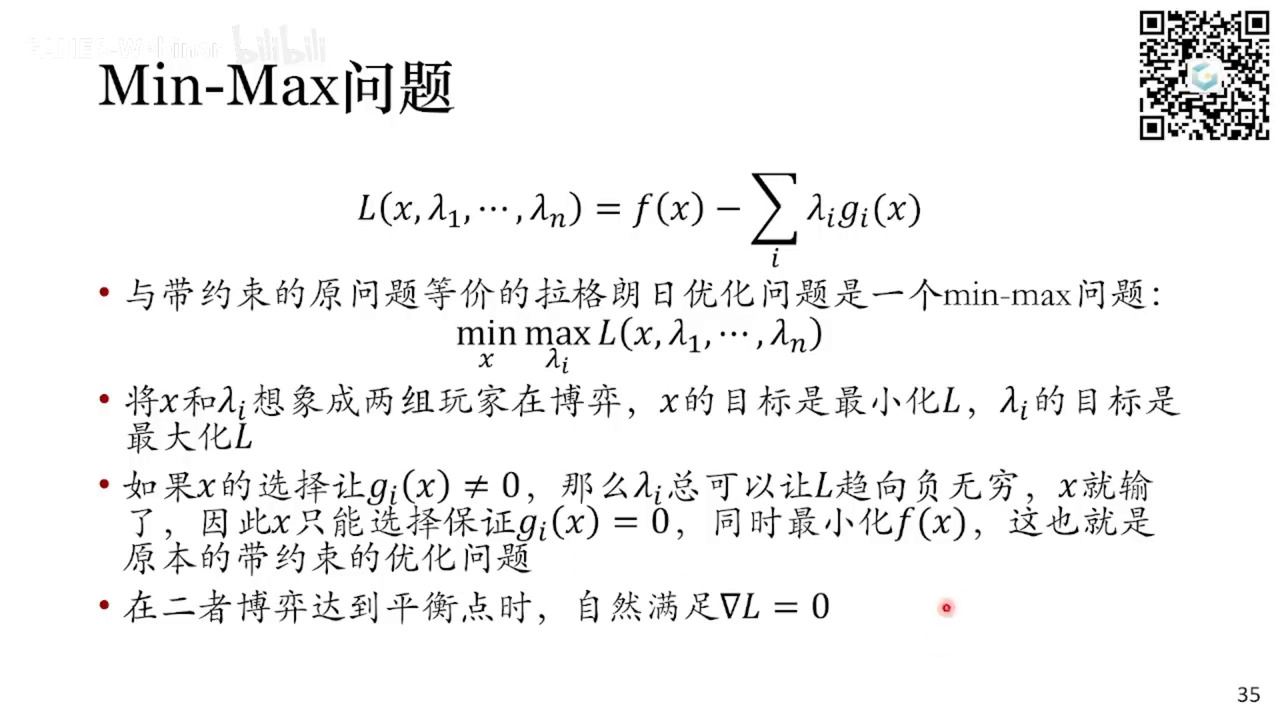
\includegraphics[width=0.92\textwidth]{figures/fig_36_minmax.jpg}
\caption{Min-Max 问题：$x$ 与 $\lambda$ 两组玩家的博弈\vtag}
\end{figure}
\srcnote{01:02:45--01:03:00}
\end{minipage}


与带约束的原问题等价的拉格朗日优化问题是一个 min-max 问题：
\begin{equation}
\min_x\max_{\lambda_i}L(x,\lambda_1,\dots,\lambda_n).
\end{equation}
讲者让大家把 $x$ 和 $\lambda_i$ 想象成两组玩家在博弈：$x$ 的目标是最小化 $L$，$\lambda_i$ 的目标是最大化 $L$。如果 $x$ 一不小心让 $g_i(x)\ne 0$，那么 $\lambda_i$ 总可以取到正无穷或负无穷，让 $L$ 趋向正无穷，$x$ 就输了。因此 $x$ 只能选择保证 $g_i(x)=0$，同时最小化 $f(x)$，这正是原本的带约束优化问题。在二者博弈达到平衡点时，自然满足 $\nabla L=0$。

\begin{warningbox}{是正无穷而不是负无穷}
课件第 35 页写的是“$\lambda_i$ 总可以让 $L$ 趋向负无穷，$x$ 就输了”。$\lambda_i$ 一方的目标是最大化 $L$，它会把 $L$ 推向正无穷，讲者口头上说的也是“趋向于正无穷”，这才是 $x$ 一方输了的意思，应以口头说法为准。上一页所说的 $L\to-\infty$ 是另一回事：那是同时对 $x$ 和 $\lambda$ 最小化 $L$ 时会出现的情况。
\end{warningbox}

\section{求解拉格朗日函数：牛顿法}

\noindent\begin{minipage}{\textwidth}
\begin{figure}[H]
\centering
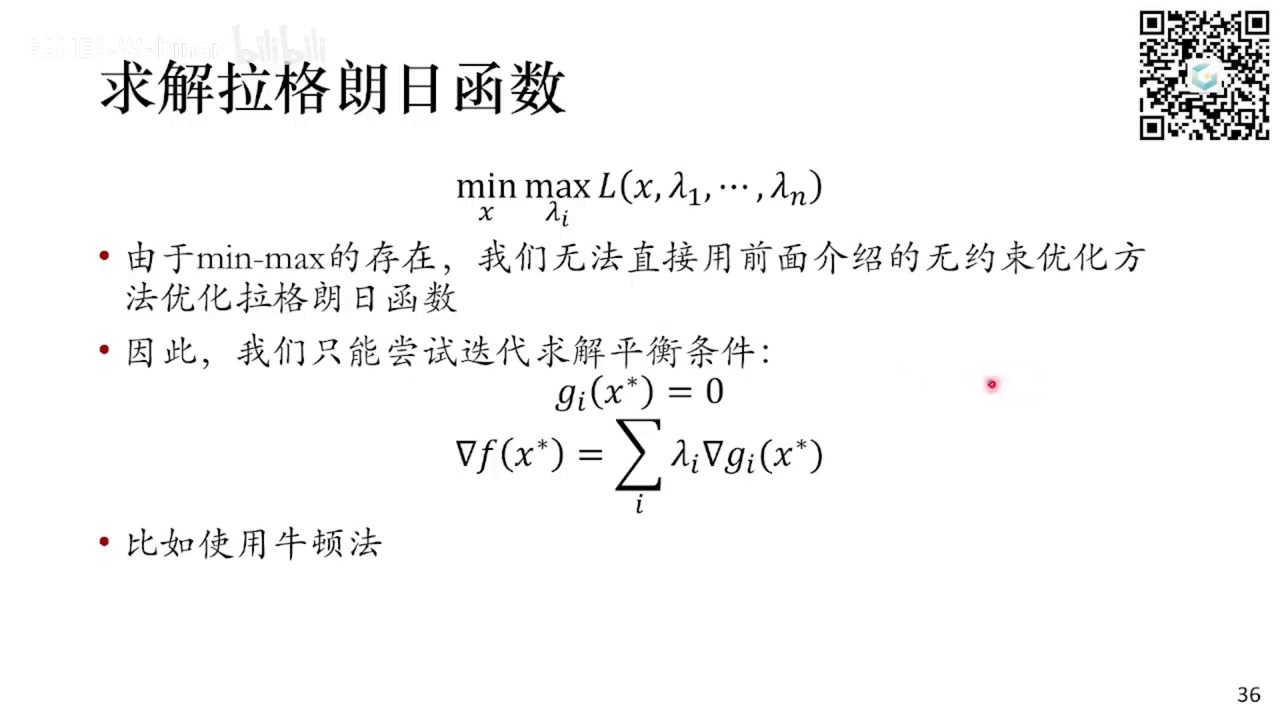
\includegraphics[width=0.92\textwidth]{figures/fig_37_solve_lagrange.jpg}
\caption{求解拉格朗日函数：迭代求解平衡条件\vtag}
\end{figure}
\srcnote{01:03:30--01:03:45}
\end{minipage}


由于 min-max 的存在，无法直接用前面介绍的无约束优化方法优化拉格朗日函数。因此只能尝试迭代求解平衡条件：
\begin{equation}
g_i(x^*)=0,\qquad \nabla f(x^*)=\sum_i\lambda_i\nabla g_i(x^*),
\end{equation}
比如使用牛顿法。

\subsection{牛顿法解方程}

\noindent\begin{minipage}{\textwidth}
\begin{figure}[H]
\centering
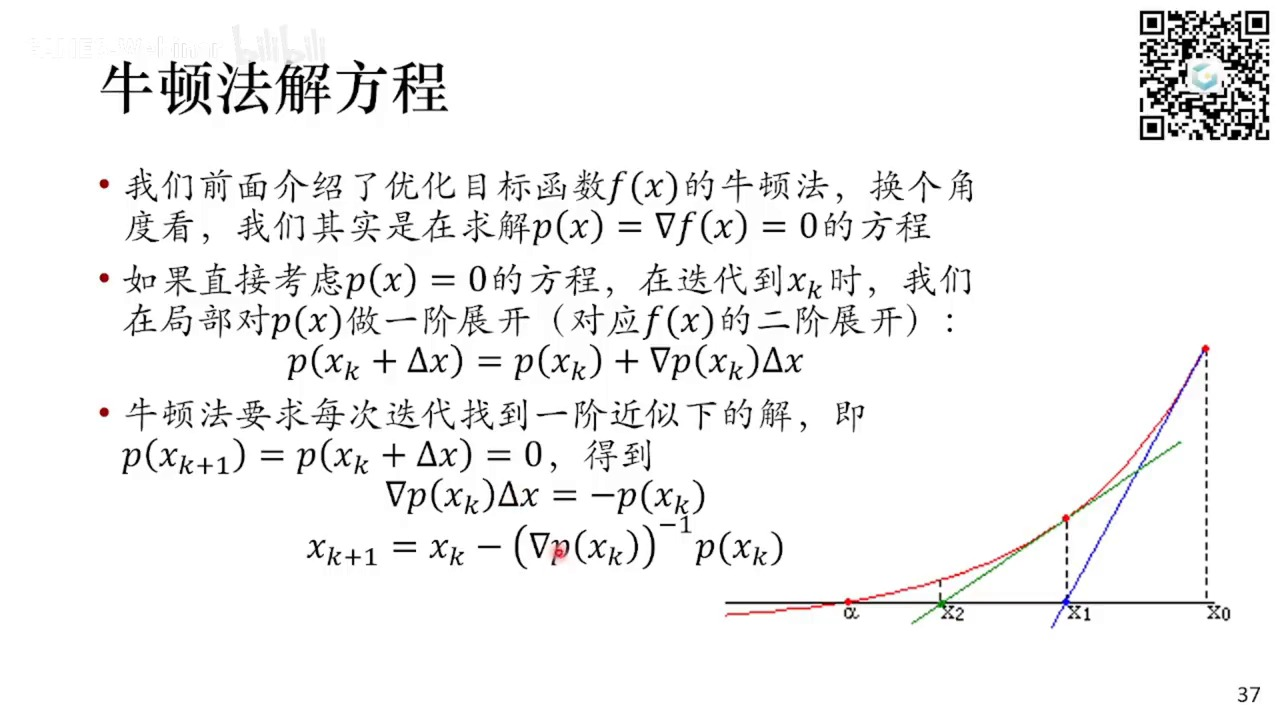
\includegraphics[width=0.92\textwidth]{figures/fig_38_newton_eq.jpg}
\caption{牛顿法解方程：局部一阶展开\vtag}
\end{figure}
\srcnote{01:06:00--01:06:15}
\end{minipage}


讲者换了个角度看前面优化 $f(x)$ 的牛顿法：它其实是在求解 $p(x)=\nabla f(x)=0$ 这个方程。如果直接考虑方程 $p(x)=0$，在迭代到 $x_k$ 时，在局部对 $p(x)$ 做一阶展开（对应 $f(x)$ 的二阶展开）：
\begin{equation}
p(x_k+\Delta x)=p(x_k)+\nabla p(x_k)\Delta x .
\end{equation}
牛顿法要求每次迭代找到一阶近似下的解，即 $p(x_{k+1})=p(x_k)+\Delta x=0$ 意义下的零点，得到
\begin{equation}
\nabla p(x_k)\Delta x=-p(x_k),\qquad x_{k+1}=x_k-\left(\nabla p(x_k)\right)^{-1}p(x_k).
\end{equation}
讲者解释：在一维的图上，就是在当前点作曲线的切线，找到切线与横轴的交点作为下一步，一直这么进行下去，最终收敛到真正的解。

\subsection{应用到拉格朗日函数}

\noindent\begin{minipage}{\textwidth}
\begin{figure}[H]
\centering
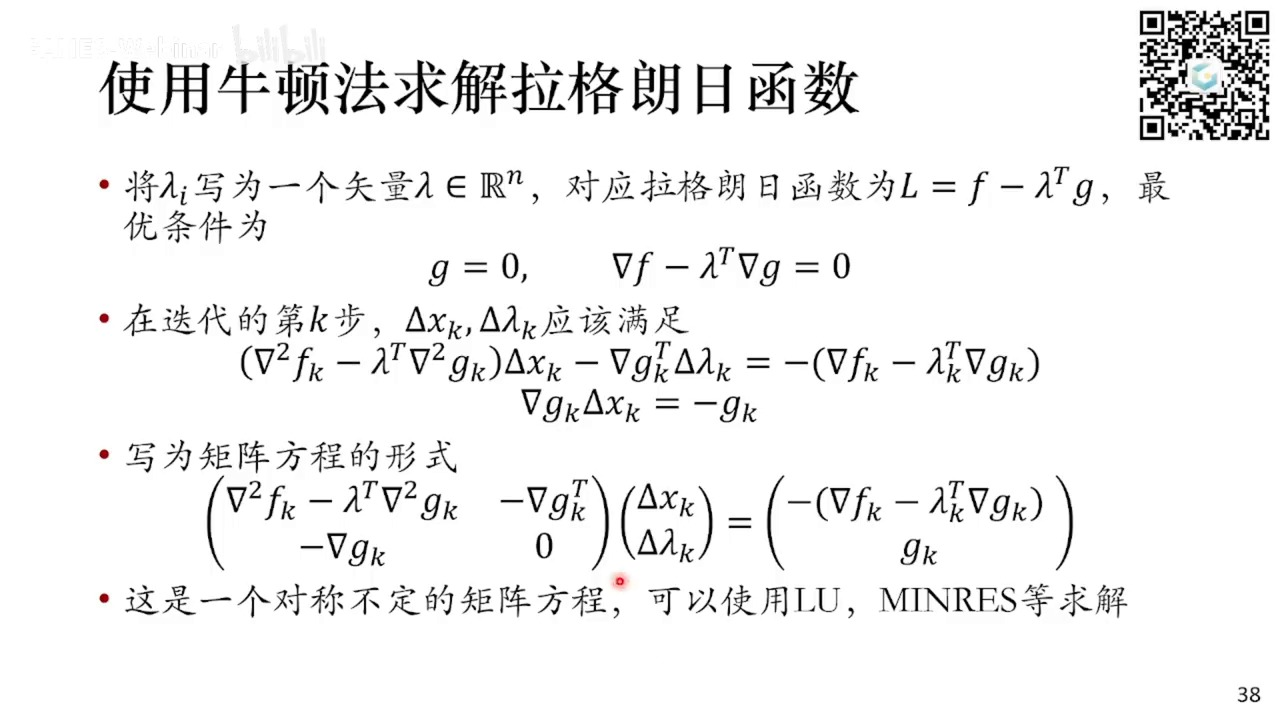
\includegraphics[width=0.92\textwidth]{figures/fig_39_newton_lagrange.jpg}
\caption{使用牛顿法求解拉格朗日函数的矩阵方程\vtag}
\end{figure}
\srcnote{01:08:30--01:08:45}
\end{minipage}


将 $\lambda_i$ 写为一个矢量 $\lambda\in\mathbb R^n$，对应拉格朗日函数 $L=f-\lambda^{\mathrm T}g$，最优条件为
\begin{equation}
g=0,\qquad \nabla f-\lambda^{\mathrm T}\nabla g=0 .
\end{equation}
在迭代的第 $k$ 步，把这两个方程在 $(x_k,\lambda_k)$ 附近做线性展开并令其为零，$\Delta x_k,\Delta\lambda_k$ 应该满足
\begin{equation}
\left(\nabla^2f_k-\lambda_k^{\mathrm T}\nabla^2g_k\right)\Delta x_k-\nabla g_k^{\mathrm T}\Delta\lambda_k=-\left(\nabla f_k-\lambda_k^{\mathrm T}\nabla g_k\right),\qquad \nabla g_k\Delta x_k=-g_k .
\end{equation}
写为矩阵方程的形式：
\begin{equation}
\begin{pmatrix}\nabla^2f_k-\lambda_k^{\mathrm T}\nabla^2g_k&-\nabla g_k^{\mathrm T}\\-\nabla g_k&0\end{pmatrix}\begin{pmatrix}\Delta x_k\\ \Delta\lambda_k\end{pmatrix}=\begin{pmatrix}-\left(\nabla f_k-\lambda_k^{\mathrm T}\nabla g_k\right)\\ g_k\end{pmatrix}.
\end{equation}
这是一个对称不定的矩阵方程，可以使用 LU、MINRES 等求解。解出后更新 $x_k$ 和 $\lambda_k$，直到收敛到平衡点。

\begin{warningbox}{这个矩阵不是正定的}
右下角是零块，所以这个“KKT 矩阵”即使左上角正定也必然有负特征值。讲义作者提醒：这意味着不能用共轭梯度、Cholesky 这类只适用于正定矩阵的快速求解器，讲者也说这种做法一般不是特别快，这正是下一节转向对偶问题的动机。
\end{warningbox}

\section{对偶问题}

\noindent\begin{minipage}{\textwidth}
\begin{figure}[H]
\centering
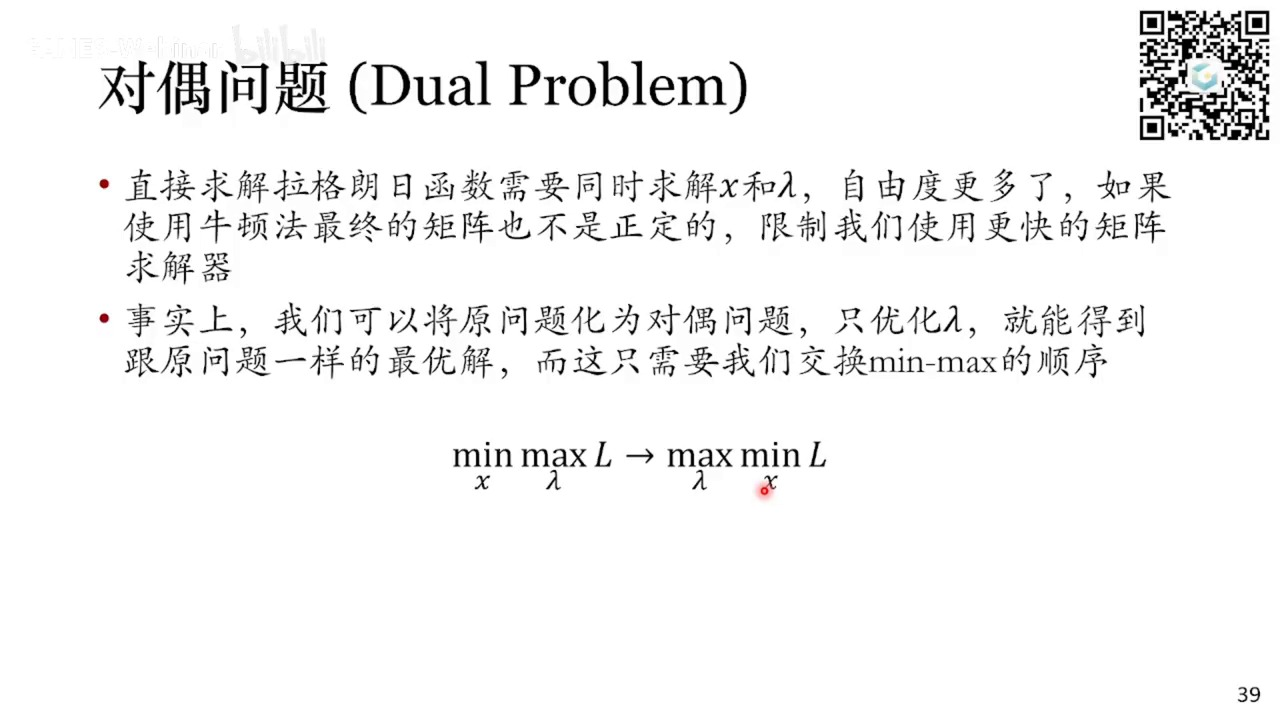
\includegraphics[width=0.92\textwidth]{figures/fig_40_dual1.jpg}
\caption{对偶问题：交换 min-max 的顺序\vtag}
\end{figure}
\srcnote{01:10:15--01:10:30}
\end{minipage}


直接求解拉格朗日函数需要同时求解 $x$ 和 $\lambda$，自由度更多了；如果使用牛顿法，最终的矩阵也不是正定的，限制了我们使用更快的矩阵求解器。事实上，可以将原问题化为对偶问题，只优化 $\lambda$，就能得到与原问题一样的最优解，而这只需要交换 min-max 的顺序：
\begin{equation}
\min_x\max_\lambda L\ \to\ \max_\lambda\min_xL .
\end{equation}
讲者用博弈来解释：原问题是 $\lambda$ 先走、$x$ 后应对；对偶问题则是 $x$ 先选，$\lambda$ 再应对，顺序交换了。

\subsection{弱对偶与强对偶}

\noindent\begin{minipage}{\textwidth}
\begin{figure}[H]
\centering
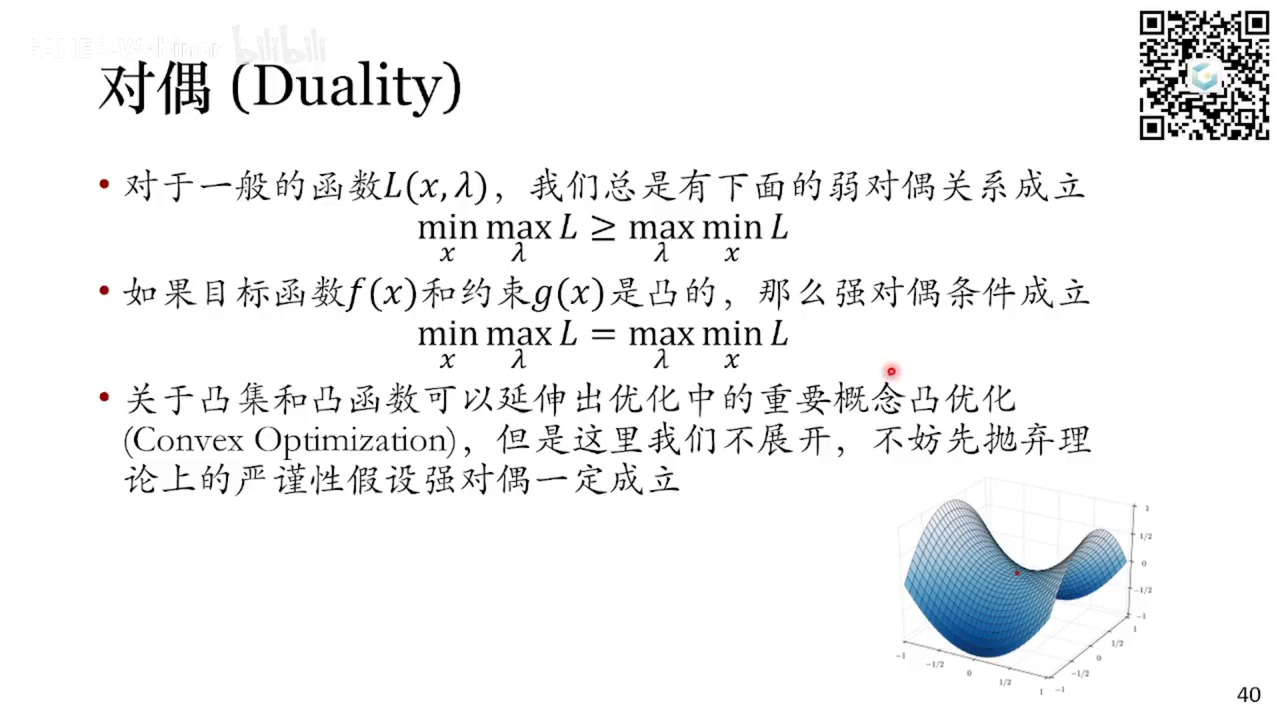
\includegraphics[width=0.92\textwidth]{figures/fig_41_duality.jpg}
\caption{对偶：弱对偶与强对偶\vtag}
\end{figure}
\srcnote{01:12:30--01:12:45}
\end{minipage}


对于一般的函数 $L(x,\lambda)$，总有下面的弱对偶关系成立：
\begin{equation}
\min_x\max_\lambda L\ \ge\ \max_\lambda\min_xL .
\end{equation}
如果目标函数 $f(x)$ 和约束 $g(x)$ 是凸的，那么强对偶条件成立，等号成立，对偶问题的最优解与原问题相等。关于凸集和凸函数，可以延伸出优化中的重要概念凸优化（convex optimization），讲者说今天没有时间展开，不妨先抛弃理论上的严谨性，假设强对偶一定成立；事实上大部分大家接触到的优化问题，做这样的对偶转换一般都是可以转换过去的。

\begin{knowledgebox}{弱对偶为什么总成立}
讲义作者补充：对任意 $x'$ 和 $\lambda'$，有 $\min_xL(x,\lambda')\le L(x',\lambda')\le\max_\lambda L(x',\lambda)$。左边与 $x'$ 无关，右边与 $\lambda'$ 无关，于是对左边取关于 $\lambda'$ 的最大、对右边取关于 $x'$ 的最小，不等式依然成立。直观地说，后行动的一方占便宜。
\end{knowledgebox}

\subsection{对偶函数}

\noindent\begin{minipage}{\textwidth}
\begin{figure}[H]
\centering
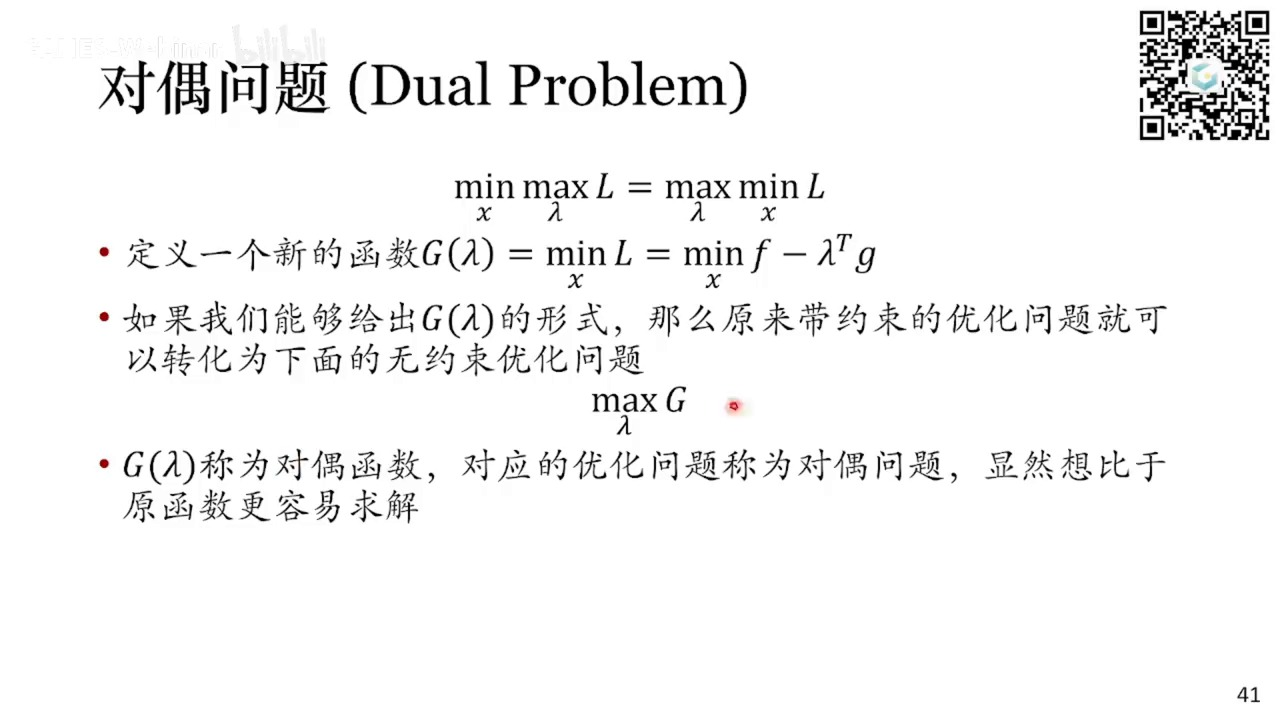
\includegraphics[width=0.92\textwidth]{figures/fig_42_dual2.jpg}
\caption{对偶函数与对偶问题\vtag}
\end{figure}
\srcnote{01:13:30--01:13:45}
\end{minipage}


定义一个新的函数
\begin{equation}
G(\lambda)=\min_xL=\min_x\left(f-\lambda^{\mathrm T}g\right).
\end{equation}
如果能够给出 $G(\lambda)$ 的形式，那么原来带约束的优化问题就可以转化为下面的无约束优化问题：
\begin{equation}
\max_\lambda G(\lambda).
\end{equation}
$G(\lambda)$ 称为对偶函数，对应的优化问题称为对偶问题，课件上说它显然比原问题更容易求解。

\subsection{一个解析的例子}

\noindent\begin{minipage}{\textwidth}
\begin{figure}[H]
\centering
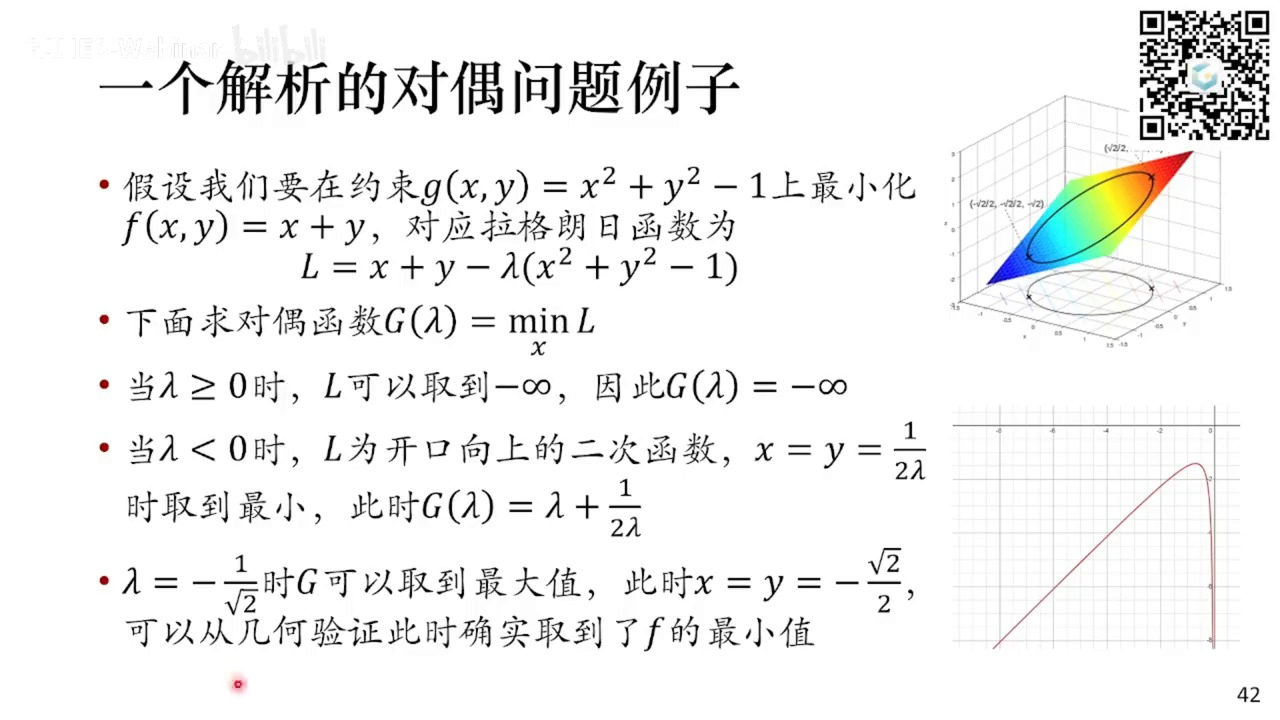
\includegraphics[width=0.92\textwidth]{figures/fig_43_dual_example.jpg}
\caption{一个解析的对偶问题例子：在单位圆上最小化 $x+y$\vtag}
\end{figure}
\srcnote{01:17:30--01:17:45}
\end{minipage}


假设要在约束 $g(x,y)=x^2+y^2-1=0$ 上最小化 $f(x,y)=x+y$，也就是让点在单位圆上运动，最小化 $x+y$。对应拉格朗日函数为
\begin{equation}
L=x+y-\lambda\left(x^2+y^2-1\right).
\end{equation}
下面求对偶函数 $G(\lambda)=\min_{x,y}L$：
\begin{itemize}
\item 当 $\lambda\ge 0$ 时，$L$ 关于 $x,y$ 是开口向下的二次函数（$\lambda=0$ 时是线性函数），可以取到 $-\infty$，因此 $G(\lambda)=-\infty$；
\item 当 $\lambda<0$ 时，$L$ 为开口向上的二次函数，在 $x=y=\frac{1}{2\lambda}$ 时取到最小，此时
\begin{equation}
G(\lambda)=\lambda+\frac{1}{2\lambda}.
\end{equation}
\end{itemize}
在 $\lambda<0$ 上最大化 $G$：令 $G'(\lambda)=1-\frac{1}{2\lambda^2}=0$，得 $\lambda=-\frac{1}{\sqrt2}$ 时 $G$ 取到最大值 $-\sqrt2$，此时 $x=y=-\frac{\sqrt2}{2}$。讲者说可以从几何上验证此时确实取到了 $f$ 的最小值：直线 $x+y=c$ 在第三象限与单位圆相切的地方，最小值正是 $-\sqrt2$，与原问题一致，强对偶在这里成立。

\section{对偶上升法与罚函数法}

\subsection{对偶上升法}

一般情况下写不出 $G(\lambda)$ 的解析形式，对偶上升法（dual ascent）利用对偶问题的形式
\begin{equation}
\max_\lambda G(\lambda)=\max_\lambda\min_xL(x,\lambda),
\end{equation}
交替更新 $x_k$ 和 $\lambda_k$。在算法的每一步，首先固定 $\lambda_k$，单独求解 $x$ 的优化问题，相当于计算 $G(\lambda_k)$：
\begin{equation}
x_{k+1}=\arg\min_xL(x,\lambda_k).
\end{equation}
然后再用梯度上升更新 $\lambda_k$：
\begin{equation}
\lambda_{k+1}=\lambda_k+\alpha_k\nabla_\lambda G,
\end{equation}
其中 $\alpha_k$ 是步长。

\noindent\begin{minipage}{\textwidth}
\begin{figure}[H]
\centering
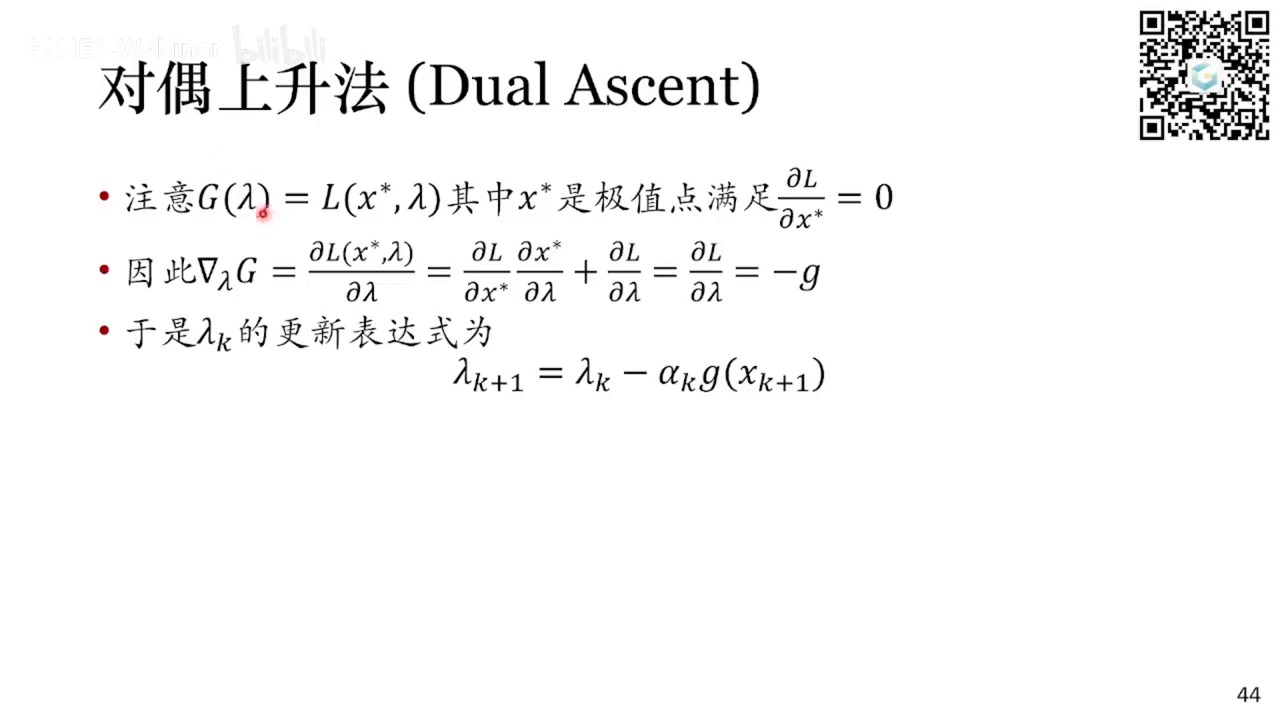
\includegraphics[width=0.92\textwidth]{figures/fig_44_dual_ascent1.jpg}
\caption{对偶上升法：交替更新 $x_k$ 和 $\lambda_k$\vtag}
\end{figure}
\srcnote{01:18:45--01:19:00}
\end{minipage}


\noindent\begin{minipage}{\textwidth}
\begin{figure}[H]
\centering
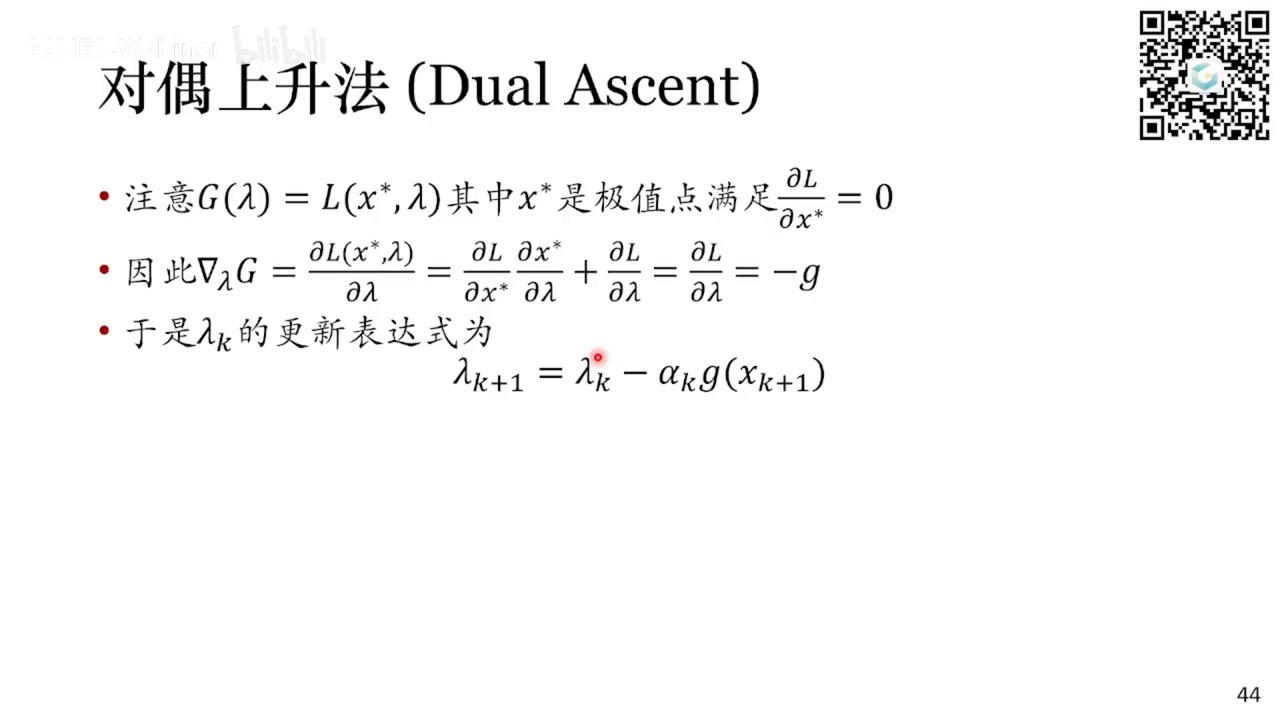
\includegraphics[width=0.92\textwidth]{figures/fig_45_dual_ascent2.jpg}
\caption{对偶函数的梯度等于 $-g$\vtag}
\end{figure}
\srcnote{01:20:45--01:21:00}
\end{minipage}


怎样求 $\nabla_\lambda G$？注意 $G(\lambda)=L(x^*,\lambda)$，其中 $x^*$ 是极值点，满足 $\frac{\partial L}{\partial x^*}=0$。用链式法则：
\begin{equation}
\nabla_\lambda G=\frac{\partial L(x^*,\lambda)}{\partial\lambda}=\frac{\partial L}{\partial x^*}\frac{\partial x^*}{\partial\lambda}+\frac{\partial L}{\partial\lambda}=\frac{\partial L}{\partial\lambda}=-g .
\end{equation}
于是 $\lambda_k$ 的更新表达式为
\begin{equation}
\lambda_{k+1}=\lambda_k-\alpha_kg(x_{k+1}).
\end{equation}
讲者总结：这样就把原问题拆成了两个无约束的优化问题，对 $\lambda$ 用梯度上升，对 $x$ 也可以用梯度法等任意无约束方法，相当于一阶方法，不需要解那个不定的矩阵方程。

\begin{importantbox}{对偶上升的直观含义}
$\lambda$ 的更新量正比于约束的违反量 $g(x_{k+1})$：约束违反得越多，乘子调整得越多，下一轮对 $x$ 的“惩罚”方向就越强；当约束被满足时 $g=0$，$\lambda$ 停止变化，算法到达平衡点。乘子可以理解为维持约束所需要的“力”。
\end{importantbox}

\subsection{罚函数法}

\noindent\begin{minipage}{\textwidth}
\begin{figure}[H]
\centering
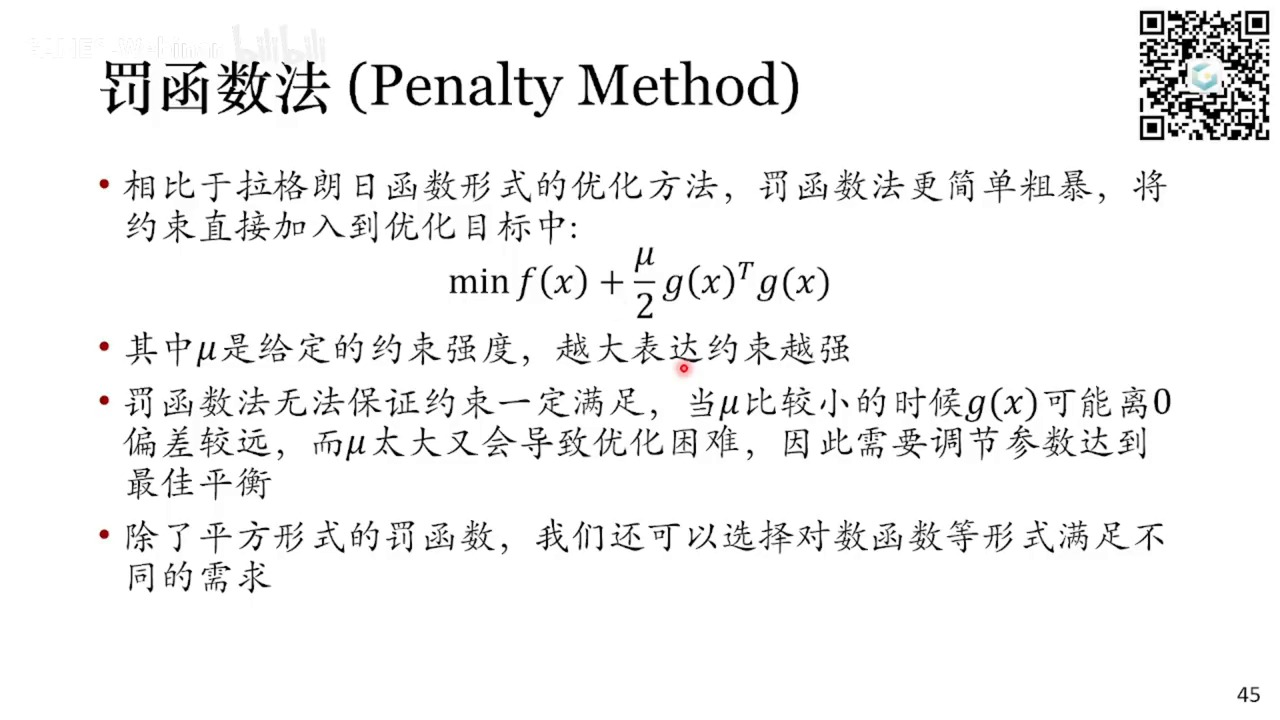
\includegraphics[width=0.92\textwidth]{figures/fig_46_penalty.jpg}
\caption{罚函数法：把约束直接加入优化目标\vtag}
\end{figure}
\srcnote{01:23:15--01:23:30}
\end{minipage}


相比于拉格朗日函数形式的优化方法，罚函数法（penalty method）更简单粗暴，将约束直接加入到优化目标中：
\begin{equation}
\min_x\ f(x)+\frac{\mu}{2}g(x)^{\mathrm T}g(x).
\end{equation}
其中 $\mu$ 是给定的约束强度，越大表示约束越强。讲者解释：如果 $\mu$ 很大，后面这一项要尽可能小，$g(x)$ 就要尽可能接近零。

罚函数法无法保证约束一定满足：当 $\mu$ 比较小时，约束很软，$g(x)$ 可能离零偏差较远；而 $\mu$ 太大又会导致优化困难，因为目标里多了一项很大的二次项。因此需要调节参数达到最佳平衡。除了平方形式的罚函数，还可以选择对数函数等形式满足不同的需求。

\begin{knowledgebox}{罚函数与增广拉格朗日}
讲义作者补充：把罚函数项与拉格朗日项合在一起，$L_\mu=f-\lambda^{\mathrm T}g+\frac{\mu}{2}g^{\mathrm T}g$，再用对偶上升的方式更新 $\lambda$，就是增广拉格朗日法。它既不需要 $\mu$ 趋于无穷就能精确满足约束，又比单纯的对偶上升收敛更稳，常与 ADMM 等算法联系在一起。
\end{knowledgebox}

\section{不等式约束}

\noindent\begin{minipage}{\textwidth}
\begin{figure}[H]
\centering
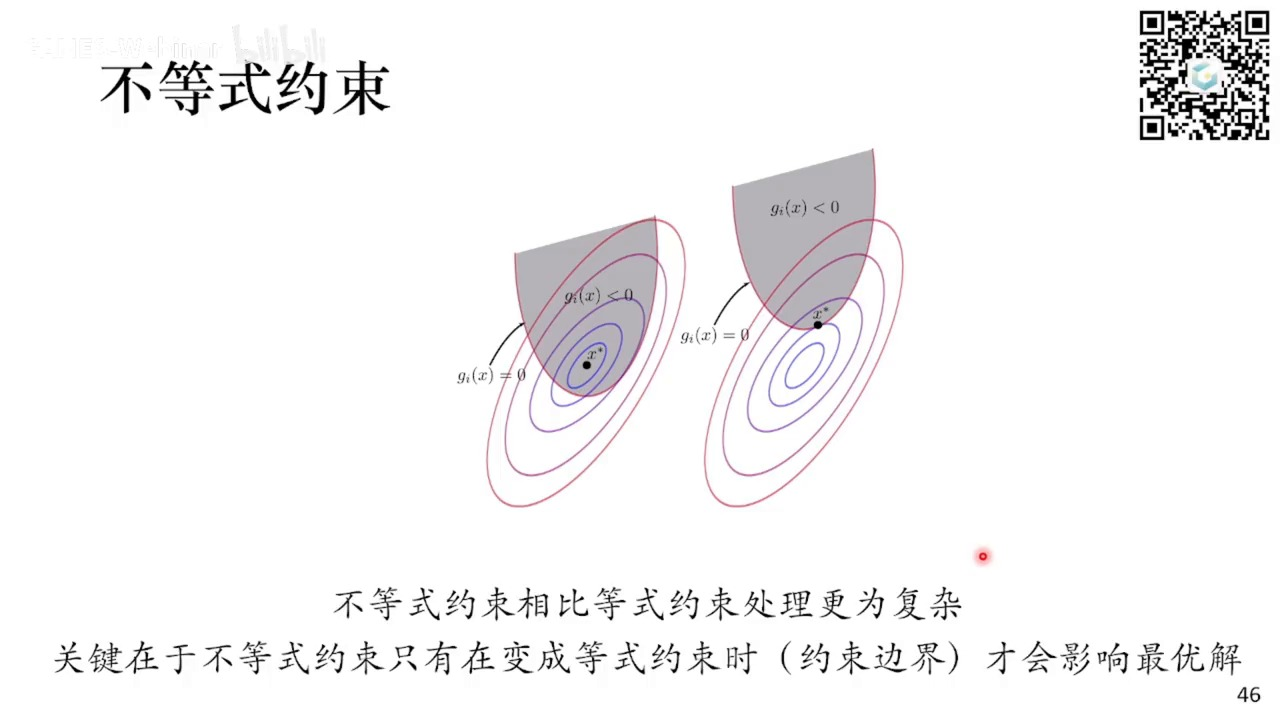
\includegraphics[width=0.92\textwidth]{figures/fig_47_ineq1.jpg}
\caption{不等式约束只在约束边界上才会影响最优解\vtag}
\end{figure}
\srcnote{01:25:30--01:25:45}
\end{minipage}


不等式约束相比等式约束处理更为复杂。关键在于不等式约束只有在变成等式约束时（约束边界）才会影响最优解。讲者解释：如果最优点在不等式约束的范围里面，那不等式约束跟没有约束是一样的；它唯一发挥作用的地方，恰恰是不等式约束变成等式约束的那条边界。如果无约束的最优解在不等式范围外面，那就把不等式约束当成等式约束一样处理。困难恰恰在于判断哪些约束是需要考虑的“起作用的约束”。

\noindent\begin{minipage}{\textwidth}
\begin{figure}[H]
\centering
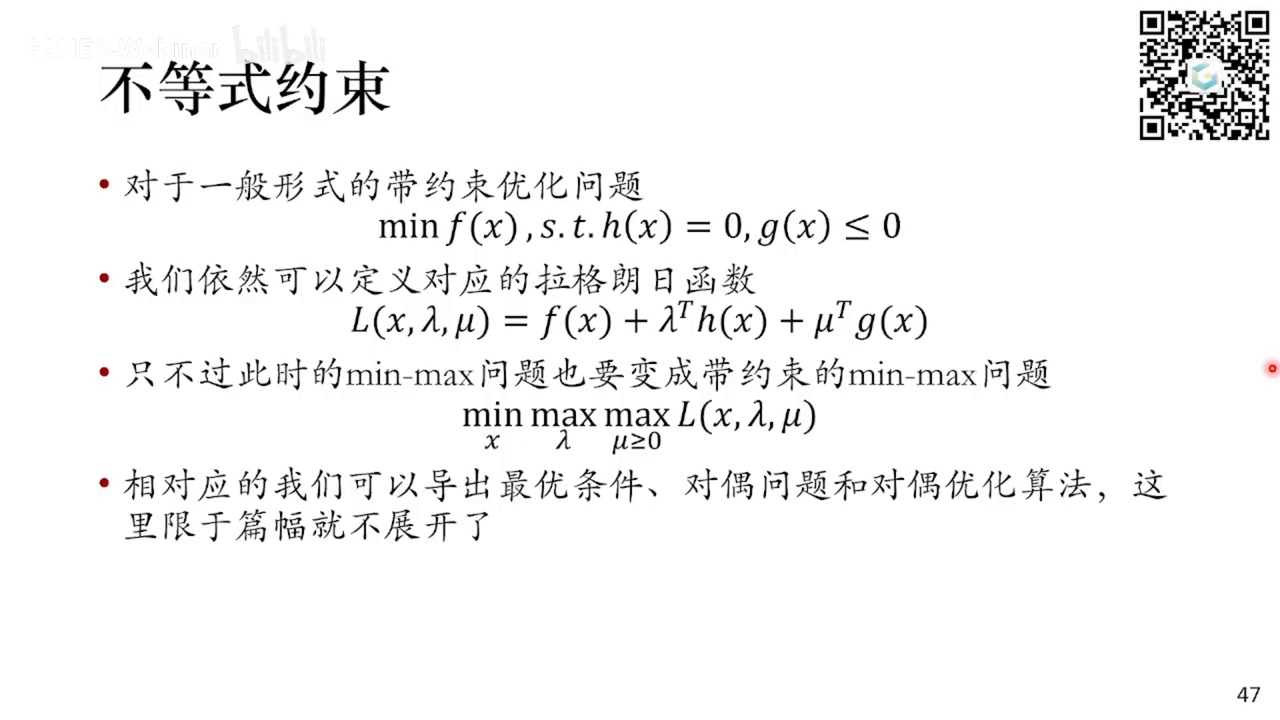
\includegraphics[width=0.92\textwidth]{figures/fig_48_ineq2.jpg}
\caption{不等式约束的拉格朗日函数与带约束的 min-max 问题\vtag}
\end{figure}
\srcnote{01:28:45--01:29:00}
\end{minipage}


对一般形式的带约束优化问题
\begin{equation}
\min f(x),\quad\mathrm{s.t.}\quad h(x)=0,\ g(x)\le 0,
\end{equation}
依然可以定义对应的拉格朗日函数
\begin{equation}
L(x,\lambda,\mu)=f(x)+\lambda^{\mathrm T}h(x)+\mu^{\mathrm T}g(x).
\end{equation}
只不过此时的 min-max 问题也要变成带约束的 min-max 问题：
\begin{equation}
\min_x\max_\lambda\max_{\mu\ge 0}L(x,\lambda,\mu).
\end{equation}
讲者解释为什么 $\mu$ 必须非负：如果 $x$ 一旦让 $g(x)$ 取到大于零的值，$\mu$ 就可以取很大的正值使得 $L$ 趋向正无穷，$x$ 就输了；所以 $x$ 想赢，一定要取 $g(x)\le 0$。只要限制了 $\mu\ge 0$ 让它参与博弈，博弈的平衡点就满足 $h(x)=0$ 和 $g(x)\le 0$ 的限制，并在此基础上让 $f(x)$ 取到最小。相应地可以导出最优条件、对偶问题和对偶优化算法，课件限于篇幅不展开。

\begin{knowledgebox}{KKT 条件}
讲义作者补充：这个带约束 min-max 问题的平衡条件就是著名的 KKT 条件：$\nabla f+\lambda^{\mathrm T}\nabla h+\mu^{\mathrm T}\nabla g=0$，$h=0$，$g\le 0$，$\mu\ge 0$，以及互补松弛 $\mu_ig_i=0$。最后一条正好表达了“不等式约束只在边界上起作用”：不在边界上时 $g_i<0$，对应 $\mu_i$ 必须为零。
\end{knowledgebox}

\section{总结}

\noindent\begin{minipage}{\textwidth}
\begin{figure}[H]
\centering
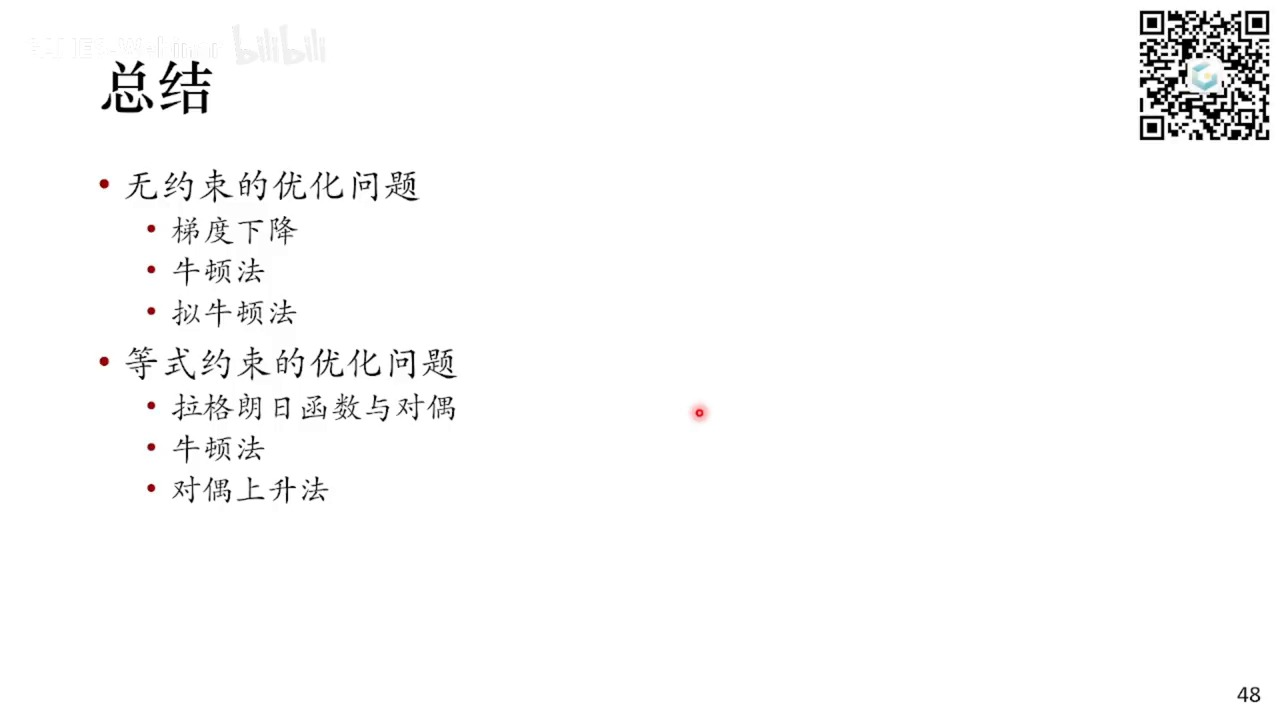
\includegraphics[width=0.92\textwidth]{figures/fig_49_summary.jpg}
\caption{总结\vtag}
\end{figure}
\srcnote{01:32:15--01:32:30}
\end{minipage}


讲者总结了今天主讲的两类问题：
\begin{itemize}
\item 无约束优化：梯度下降法、牛顿法、拟牛顿法。梯度下降只用一阶信息，配合 Armijo 条件的线搜索；牛顿法利用二阶信息，收敛快但要解海森矩阵方程，并要处理不正定的情况；拟牛顿法用近似矩阵代替海森矩阵，BFGS 和 L-BFGS 是最常用的选择。
\item 等式约束优化：拉格朗日函数与对偶的概念，讨论了等式约束问题在什么情况下取到最优，以及为什么不能直接最小化拉格朗日函数；然后用牛顿法求解平衡条件，或者转化为对偶问题，用对偶上升法轮流迭代 $x$ 与乘子，让它收敛到最终的平衡解。
\end{itemize}
讲者说今天没讲到的东西非常多，比如带不等式约束的迭代方法、离散空间上的优化等等；如果大家遇到更难的问题，或者需要更快的优化算法，可以再进一步深入地学习优化相关的知识。优化本身是一门内容分量非常大的课程，今天讲得比较多也比较快，没搞清楚的地方可以再去看看回放。

\noindent\begin{minipage}{\textwidth}
\begin{figure}[H]
\centering
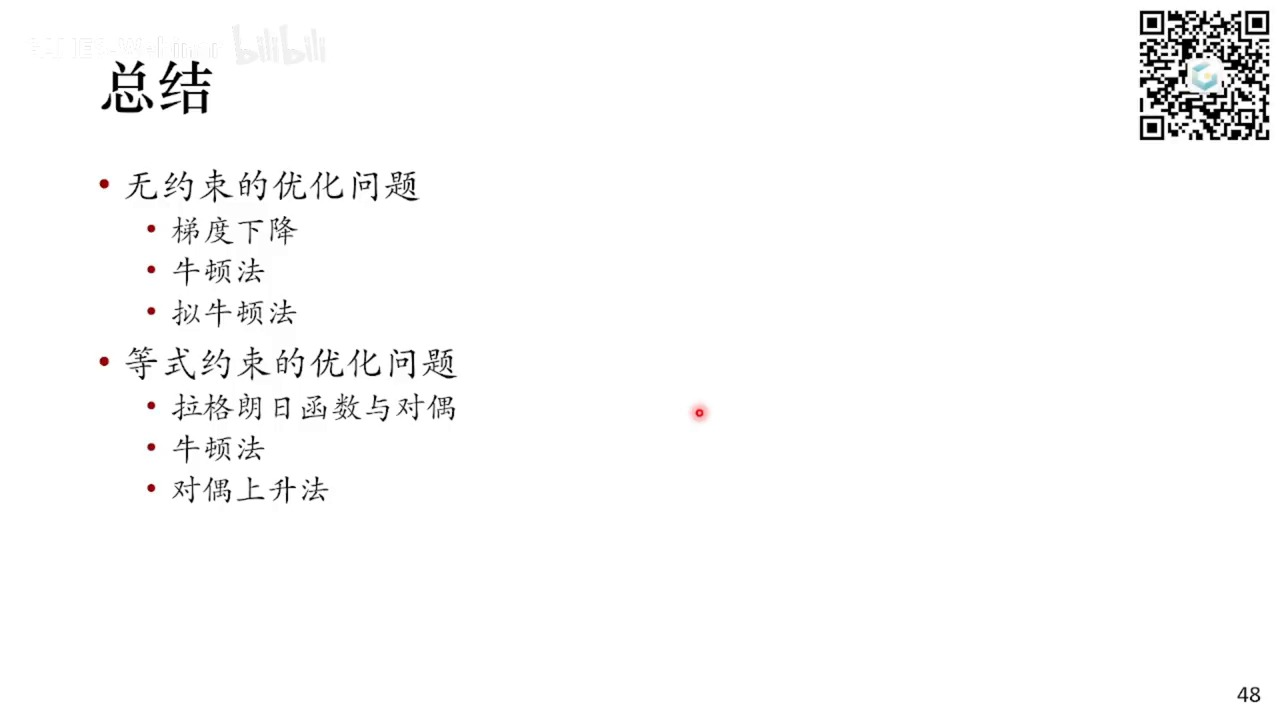
\includegraphics[width=0.92\textwidth]{figures/fig_50_references.jpg}
\caption{参考材料\vtag}
\end{figure}
\srcnote{01:32:15--01:32:30}
\end{minipage}


课件给出的参考材料包括《An Introduction to Optimization Techniques in Computer Graphics》、《Introduction to Mathematical Optimization with Python》、一个连续优化的在线教程、《BFGS in a Nutshell: An Introduction to Quasi-Newton Methods》、一门计算机图形学中的优化课程主页，以及 GeometricOptimization 代码仓库。

\begin{practicebox}{自测}
\begin{enumerate}
\item 写出 Armijo 条件，并解释为什么回溯线搜索要从较大的步长（例如 $1$）开始减小。
\item 当海森矩阵不正定时，牛顿方向可能不是下降方向。请用二次型解释原因，并给出两种处理办法。
\item 验证 BFGS 更新后的 $\mathbf B_{k+1}$ 满足割线条件 $\mathbf B_{k+1}s_k=y_k$。
\item 对“在单位圆上最小化 $x+y$”的例子，验证对偶函数最大值等于原问题最小值。
\item 比较罚函数法与对偶上升法在约束满足程度和参数调节上的差别。
\end{enumerate}
\end{practicebox}

\end{document}
